\documentclass[a4paper, 12pt]{article}
% Allow the usage of graphics (.png, .jpg)
\usepackage[pdftex]{graphicx}
\graphicspath{ {./images/} }
\usepackage{apacite}
\usepackage[T1]{fontenc}
\usepackage{url}
\usepackage{amsmath}
\usepackage{algorithm}
\usepackage{algpseudocode}
\usepackage{subcaption}
\usepackage{float}
\usepackage{multirow}

\makeatletter
\def\BState{\State\hskip-\ALG@thistlm}
\renewcommand{\ALG@name}{Convert to OF}
\renewcommand{\thealgorithm}{}
\makeatother

% set line spacing
\usepackage{setspace}
\setlength{\parindent}{0pt}
\setlength{\parskip}{2ex}
\linespread{1.3}

% caption
\usepackage{caption} 
\captionsetup[table]{skip=10pt}

\usepackage{tocloft} % for list of equations
% define list of equations
\newcommand{\listequationsname}{\Large{List of Equations}}
\newlistof{myequations}{equ}{\listequationsname}
\newcommand{\myequations}[1]{
   \addcontentsline{equ}{myequations}{\protect\numberline{\theequation}#1}
}
\setlength{\cftmyequationsnumwidth}{2.3em}
\setlength{\cftmyequationsindent}{1.5em}

% Comment the following line to NOT allow the usage of umlauts
\usepackage[utf8]{inputenc}
%custom margins
\usepackage[]{vmargin}
\setpapersize{A4}	
\setmarginsrb{35mm}{30mm}{30mm}{20mm}{0pt}{0mm}{12pt}{13mm}
% Correct hyphenation in urls
\usepackage{url}
% Support long tables
\usepackage[]{longtable}
\usepackage{ltablex}
\usepackage{adjustbox}
%Pretty bibliography in UEF format
\usepackage{natbib}
% verbatim code listings
\usepackage{listings}
%Unobtrusive in document links
\usepackage{hyperref}
\hypersetup{
    colorlinks,
    citecolor=black,
    filecolor=black,
    linkcolor=black,
    urlcolor=black
}
%%%%%%%%%%%%%%%%%%%%%%%%%%UEF FORMAT%%%%%%%%%%%%%%%%%%%%%%%%%%%%%%%%%


\begin{document}

% do cover pages
%Fill these in and they'll propagate across the title page. Remember to keep the space at the end!
\def \ajankohta {Tammikuu 2014 }
\def \ajankohtaenglish {August 2021 }
\def \authorname {Nguyen To }
\def \thesistitle {Sign Language Recognition }
\def \thesissubtext {Inflated 3D ConvNet  }
\def \campus {Joensuu }
\def \facultyschooleng {School of Computer Science }
\def \facultyschoolfin { }
%FT = PhD, FM = MSc
\def \supervisorsfin { }
\def \supervisorseng {Profressor Xiao-Zhi Gao }

\def \documenttypeeng {Master's Thesis }
\def \documenttypefin { }
%\def \documenttypeeng {Bachelor's Thesis}
%\def \thesistypefin {Kandidaatintutkielma}

%Number of non-cover pages, to last page of references
\def \mypagecount {42 }
\def \myappendixcount {1 }
\def \myappendixpagecount {32 }

\graphicspath{ {./images/} }
%%%%%%%%%%%%%%%%%% TITLE PAGE %%%%%%%%%%%%%%%%%%

\vspace*{3cm}
\vspace{0.5cm}

\begin{center}
\begin{LARGE}\thesistitle \end{LARGE}

\begin{Large}\thesissubtext \end{Large} 

\vspace{1.5cm}

\begin{Large}\authorname \end{Large}

\vspace{\stretch{1}}

{\large
\documenttypeeng
~\\
% to have it in black and white, swap the commented line
\includegraphics[width=7cm]{{UEF logo.png}}\\
% \includegraphics[width=7cm]{UEF_fin_pysty_1_black}\\
Faculty of Science and Forestry\\
\facultyschooleng \\
}
\end{center}

\vspace{0.5cm}

\thispagestyle{empty}

\begin{spacing}{1.0}
\newpage

%%%%%%%%%%%%%%%%%% Abstract page in English %%%%%%%%%%%%%%%%%%

UNIVERSITY OF EASTERN FINLAND, Faculty of Science and Forestry, \campus School of Computing\\
\facultyschooleng \\ \\
Student, \authorname : \thesistitle \\
\documenttypeeng , \mypagecount p.\\
Supervisors of the \documenttypeeng : \supervisorseng \\
\ajankohtaenglish \\


Abstract:

Effective communication is considered as the foremost fundamental of human skills. However, more than 5\% of the world's population is suffering from disabling hearing loss, as indicated by the World Health Organization (WHO). There is hence a communication gap between the hearing-impaired community, whose primary means of communication is sign language, and others who are not privy with this language. To this end, Sign Language Recognition could be an essential instrument which utilizing vision-based technology and helps the hearing-impaired communicate with the society with ease, thereby diminishing the verbal exchange barrier. The first step in interpreting and analyzing communication via gestures is word-level sign language recognition (WSLR). Recognizing signs from recordings maybe a tough challenge due to the fact that the meaning of a word is determined by a combination of subtle body movements, hand gestures, and other actions. Be that as it may, with the significant advancement of technology, notably Convolutional Neural Network (CNN), in this paper, an Inflated 3D Networks (I3D), a 3D video categorization solution are used to method as an answer of WSLR.


% Key words English

% Edellisellä sivulla olevien suomenkielisten avainsanojen käännökset

~\\ % Tämä tekee tyhjän rivin; älä editoi tätä pois
Keywords:
Sign Language, Continuous Sign Language, Sign Language Recognition, Classification,
Vidieo Classification, Recognition

% CR-luokat

% ACM-luokitus löytyy Computing Reviews -lehden jokaisen
% vuosikerran ensimmäisestä numerosta sekä verkosta
% osoitteesta http://www.acm.org/class/

% Ota omat luokkasi tuoreimmasta vuosikerrasta.

CR Categories (ACM Computing Classification System,
1998 version): A.m, K.3.2\\

\end{spacing}

\newpage


%%%%%%%%%%%%%%%%%% Foreword/Preface %%%%%%%%%%%%%%%%%%

\section*{Preface}
The basis for the project initially originated from my ardor for developing better methods of sign language recognition. The hearing-impaired community's life has changed considerably over the past half-century as a result of policy adjustments and latest technological tendencies, yet the road to find a viable answer for word-level sign language recognition (WSLR) keeps on being a drawn out circumstance. It is my passion to not solely find out, however to develop tools to bridge the communication gap between the deaf community and the society. This project follows the reference and citation guidelines of the "Quo Valdis, Action Recognition? A New Model and the Kinetics Datasets” by a group of Jo\~{a}o Carreira and Andrew Zisserman.

In truth, I could not have achieved my current level of success without a strong support group. To begin with, I wish to express my sincere thanks to my supervisor, Profressor Xiao-Zhi Gao, for his excellent guidance, valuable input and support throughout the entire period.
Furthermore, I would also like to thank Li Dongxu for his enormously valued assistance in collecting data for this study.
Especially with respect Cong Phan, a Phd candidate at Griffith University who gave a great help by offering several useful insights and recommendations. 
And finally, I am grateful to Mai Khanh Nguyen Ngoc. She stood by my side and provided me with the support I needed to complete this thesis. 
\newpage

%%%%%%%%%%%%%%%%%% Abbrieviations %%%%%%%%%%%%%%%%%%

\section*{List of Abbreviations}

\begin{tabular}{lp{12.5cm}}

ACM & Association for Computing Machinery \\

ISY & Itä-Suomen yliopisto \\

UEF & University of Eastern Finland\\

WSLR & Word-level Sign Language Recognition\\

I3D & Two -Stream Inflated 3D Convolutional Network\\

CNN & Convolutional Neural Network\\

LSTM & Long-short Term Memory\\

TGCN & Temporal Graph Convolutional Network\\

\end{tabular}

\newpage


% ----------------- Table of Contents -------------

% Älä tee seuraavaan mitään muutoksia:

\setlength{\parskip}{0ex}

\tableofcontents
\newpage

\listoftables
\newpage

\listoffigures
\newpage

\setlength{\parskip}{2ex}

\pagenumbering{gobble} % arabic(1234) numbering, autoreset to 1


\section{Introduction}
Sign Language, any methods of communicating by bodily motions, particularly with hands and arms, that is utilized when verbal communication is either difficult or undesirable. Sign language can consist of a series of overly-exaggerated facial expressions, shrugs, or hand gestures; or it can be a fine and delicate mix of hand signals that are complemented by facial expressions and words spelt out using a manual alphabet. When a deaf person or someone speaking a different language is communicating with someone who is hearing, using sign language can help connect the parties. \citep{signlanguagedefinition2020}. The public has neither the time nor the patience to learn sign language, which is complicated and time-consuming to learn and practice. Additionally, there are also many language and culture-specific \citep{holtz2014reading} (e.g Germany, Japanese) constraints which will hinder the widespread adoption of sign language.
Significant advances in deep learning (DL) and improvements in device capabilities, such as computation power, memory capacity, power usage, sensor resolution, and optics, have improved the performance and cost-effectiveness of vision-based applications, allowing them to spread more quickly in the market place.
For this reason, it is interesting to examine sign language recognition (SLR), which automatically translates sign language and aids deaf-mute individuals in communicating with others in their life

Back to the history of 90s, Yann LeCun et al. published "Gradient-Based Learning Applied to Document Recognition", which is widely considered to be the most popular AI article from the era. This paper was the first modern application of convolutional neural networks to be developed.
Since then, more and more sophisticated models trained on ever-larger datasets have been built using the convenient approach of convolutional neural networks. Especially in the field of Computer Vision - Human-based activity recognition, there are many methods can be applied to solve the problem, from traditional convolutional neural networks such as CNN-RNN, CNN-LSTM to RestNetCRNN, Conv3D and state-of-the-art networks e.g Pose-TGCN, I3D.
Inheriting the idea of using two-stream I3D network, which is based 2D ConvNet \citep{carreira2017quo}, presented by Carreira and Zisserman, this project is re-implement the model with a slightly modification inside. It might not be better when comparing with other models, however during the project, I have got many experience and broaden my knowledge on the field of Deep Learning. 

\subsection{Problem}
As same as other human-based activity recognition, SRL also shares some common problems such as background clutter, lightning or lightning changing in a video, motion blur, angle of camera, changing scale. 
SRL, on the other hand, is a more difficult task than ordinary action recognition. Firstly, sign language relies on a combination of global body movement and subtle hand/arm gesture. Additionally, depending on how many times they are repeated, same gestures might have different meanings. SRL might be more difficult to examine because of different states of motions and signers such as localism, gesture speed, preferred hand or physical form. Finally, it is also expensive to collect additional data from many signers even though it is desirable \citep{jiang2021skeleton}.

As described above, the datasets that uses for training SLR are limited, even the number of samples inside each dataset. The table below describes some datasets that normally use for researching.

\begin{table}[ht!]
    \centering
    \def\arraystretch{1}%
    \caption{Sign Language Datasets.}
    \resizebox{\textwidth}{!}{
        \begin{tabular}{|l|l|l|l|l|l|}
            \hline \textbf{Dataset} & \textbf{Language} & \textbf{Classes} & \textbf{Samples} & \textbf{Data Type} & \textbf{Language Level} \\
            \hline CSL Dataset I & Chinese & 500 & 125,000 & Video \& Depth from Kinect & Isolated \\
            \hline CSL Dataset II & Chinese & 100 & 25,000 & Videos \& Depth from Kinect & Continuous \\
            \hline RWTH-PHOENIX-Weather 2014 & German & 1,081 & 6,841 & Videos & Continuous \\
            \hline RWTH-PHOENIX-Weather 2014 T & German & 1,066 & 8,257 & Videos & Continuous \\
            \hline ASLLVD & American & 3,300 & 9,800 & Videos(multiple angles) & Isolated \\
            \hline ASLLVD-Skeleton & American & 3,300 & 9,800 & Skeleton & Isolated \\
            \hline SIGNUM & German & 450 & 33,210 & Videos & Continuous \\
            \hline DGS Kinect 40 & German & 40 & 3,000 & Videos(multiple angles) & Isolated \\
            \hline DEVISIGN-G & Chinese & 36 & 432 & Videos & Isolated \\
            \hline DEVISIGN-D & Chinese & 500 & 6,000 & Videos & Isolated \\
            \hline DEVISIGN-L & Chinese & 2000 & 24,000 & Videos & Isolated \\
            \hline LSA64 & Argentinian & 64 & 3,200 & Videos & Isolated \\
            \hline GSL isol. & Greek & 310 & 40,785 & Videos \& Depth from RealSense & Isolated \\
            \hline GSL SD & Greek & 310 & 10,290 & Videos \& Depth from RealSense & Continuous \\
            \hline GSL SI & Greek & 310 & 10,290 & Videos \& Depth from RealSense & Continuous \\
            \hline IIITA -ROBITA & Indian & 23 & 605 & Videos & Isolated \\
            \hline PSL Kinect & Polish & 30 & 300 & Videos \& Depth from Kinect & Isolated \\
            \hline PSL ToF & Polish & 84 & 1,680 & Videos \& Depth from ToF camera & Isolated \\
            \hline BUHMAP-DB & Turkish & 8 & 440 & Videos & Isolated \\
            \hline LSE-Sign & Spanish & 2,400 & 2,400 & Videos & Isolated \\
            \hline Purdue RVL-SLLL & American & 39 & 546 & Videos & Isolated \\
            \hline RWTH-BOSTON-50 & American & 50 & 483 & Videos(multiple angles) & Isolated \\
            \hline RWTH-BOSTON-104 & American & 104 & 201 & Videos(multiple angles) & Continuous \\
            \hline RWTH-BOSTON-400 & American & 400 & 843 & Videos & Continuous \\
            \hline WLASL & American & 2,000 & 21,083 & Videos & Isolated \\
            \hline
        \end{tabular}
    }
    \label{Table dataset}
\end{table}

Time segmentation is another issue for SLR as it is difficult to distinguish different kinds of sign language while signers make gestures continuously to describe a phrase or a sentence \citep{xiao2020multi}.
Word-level sign recognition, an integral part of comprehending sign language phrases and sentences, is also extremely difficult task itself:
\begin{itemize}
    \item The meaning of signals is primarily determined by the mix of bhand actions, body motions and head positions, and small variations in these elements can result in a variety of interpretations.
    \item With the same gesture, depend on the natural languages and context, they might have different meaning. It is also possible for nouns and verbs from the same lemma to share the same sign. These nuances are not effectively reflected by the small-scale datasets that are currently available (Figure 1) \citep{li2020word}.
    \item The number of signs that are used on daily basis is enormous, it could be thousands. In comparison, tasks such as gesture and action recognition have just had a few hundred categories. The scalability of recognition algorithms is significantly hampered as a result.
\end{itemize}

\begin{figure}[H]
    \centering
    \begin{subfigure}[b]{0.3\textwidth}
        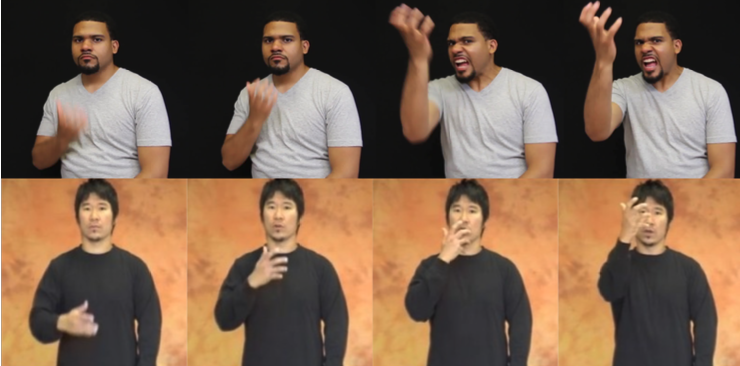
\includegraphics[width=\textwidth]{fig2a.png}
        \caption{\textbf{"Scream"} is performed slightly different by different signers}
    \end{subfigure}
    \hfill
    \begin{subfigure}[b]{0.3\textwidth}
        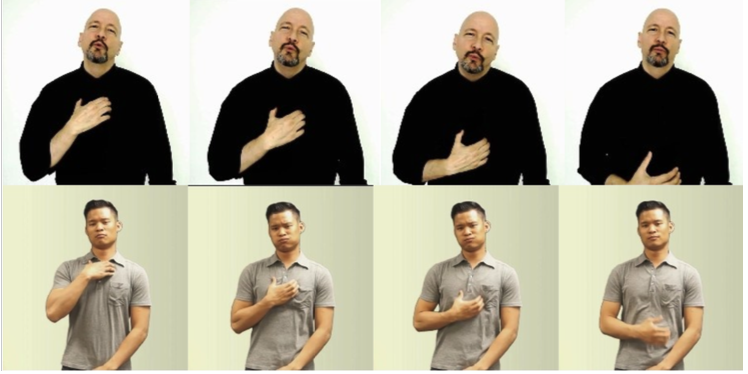
\includegraphics[width=\textwidth]{fig2b.png}
        \caption{The verb \textbf{"Wish"} (top) and the adjective \textbf{"Hungry"} (bottom) have same gesture}
    \end{subfigure}
    \hfill
    \begin{subfigure}[b]{0.3\textwidth}
        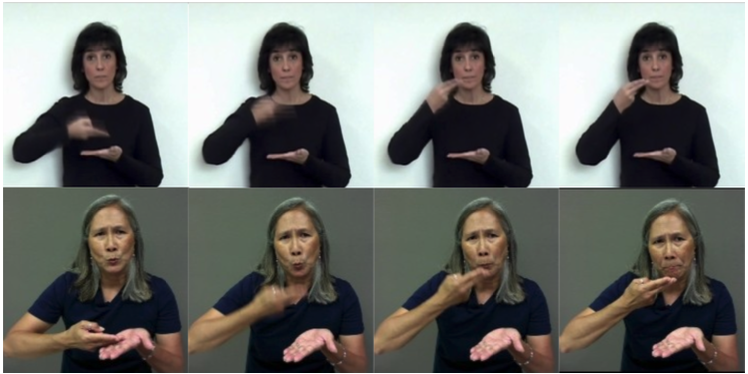
\includegraphics[width=\textwidth]{fig2c.png}
        \caption{\textbf{"Rice"} (top) and \textbf{"Soup"} (bottom) have same gesture}
    \end{subfigure}
    \caption{Common occurrence of ambiguity and variation signing}
    \label{Example of Sign language problems}
\end{figure}

\subsection{Thesis scope and target}
In fact, the researching of SLR, including isolated (word-level) and continuous (phrase or sentences), has yielded significant results and developed rapidly in recent years \Citep{lim2019isolated,li2018deep,mercanoglu2021chalearn}.
So this project aims to understand the architecture of I3D model, focuses on the methodology of training, evaluating the network with given dataset. A further objective of the project is getting familiar with libraries and frameworks of Deep Learning which is built for Python environment, and also other related topics such as image processing, data labelling, development tools e.g Google Colab, Anaconda, Jupyter Notebook.
Regarding data and dataset, the project gave a comprehensive overview of organizing data, loading, splitting data for training and testing purpose.

Finally, in terms of the topic's aim, this thesis primarily focuses on enhancing the accuracy of the dataset with the two-stream I3D network. Because of the limitation of facilities, such as hardware, and time-consuming of training process, the project only used the WLASL and ASL dataset. 
In order to reduce the consumption of training time, as well as to test the effectiveness of I3D network, the dataset is divided into many sub-datasets which have 100 classes, 300 classes, 1000 classes and 2000 classes which is applied for WLASL. Regarding ASL dataset, because the number of class is small (64 words) so this is not splitted.

\section{Model}
\subsection{Methodology of video classification and CNNs}
A video is a collection of multi images which are represented by sequential. Therefore, the main idea of clarifying an action or object inside a video is analyzing frame by frame. In details, the general procedure of video recognition \citep{sivic2003video,niebles2010modeling} contains three key stages. 
The video is first divided into regions \citep{liu2009recognizing} based on the places that are easy to characterize in visual terms. This is done by either sampling regions densely \citep{wang2013action} or, if there are few areas of interest \citep{laptev2005space}, by using a sparse sampling technique. 
In the next step, the characteristics are merged into a video level description with defined size. One common method is to train a K-means dictionary and then evaluate all the features. This allows to gather visual words during the duration of the video and then arrange them into histograms of various spatio-temporal positions and extents \citep{karpathy2014large,laptev2008learning}.
Finally, a classifier (such as an SVM) is trained to discriminate between the classes of interest with the resulting "bag of words.".

CNN, a single neural network which emulates the process of human brain \citep{lecun1998gradient} offer an approach that combines 3 phases into an end-to-end training from the raw value of pixels to the output classifiers. By using restricted connection across layers (local filters), parameter sharing (convolutions), and specific local invariance-building neurons (max pooling), the spatial structure of pictures is specifically exploited. Recently with the outstanding of GPU, CNNs can now scale the networks with millions variables, resulting in significant developments in object recognition \citep{girshick2014rich}, image classification \citep{krizhevsky2017imagenet}, scene annotation. The use of CNNs has piqued the interest of many in the computer vision research community \citep{zha2015exploiting}, and it has been demonstrated that CNN-based methods can reach state-of-the-art performance on various of complex image datasets \citep{sharif2014cnn}.

\begin{figure}[H]
    \centering
    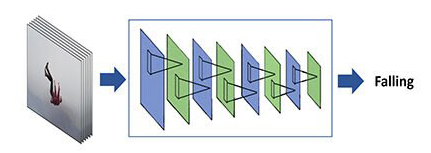
\includegraphics[width=1\textwidth]{Video_classification_and_human_activity_recognition.jpg}
    \caption{An example of video classification}
    \label{Figure of video classification}
\end{figure}

\subsection{Some models to solve video recognition problems}
\subsubsection{ConvNet-LSTM}
LSTM network and CNNs have been researched widely but independently previously. While CNNs are able to give spatially specific information, LSTM networks are good at producing temporally comprehensive results \citep{mutegeki2020cnn}. As a result, the use of CNN-LSTM networks is extensively employed for time series data, and is particularly useful for video datasets that have a time dimension.

\begin{figure}[H]
    \centering
    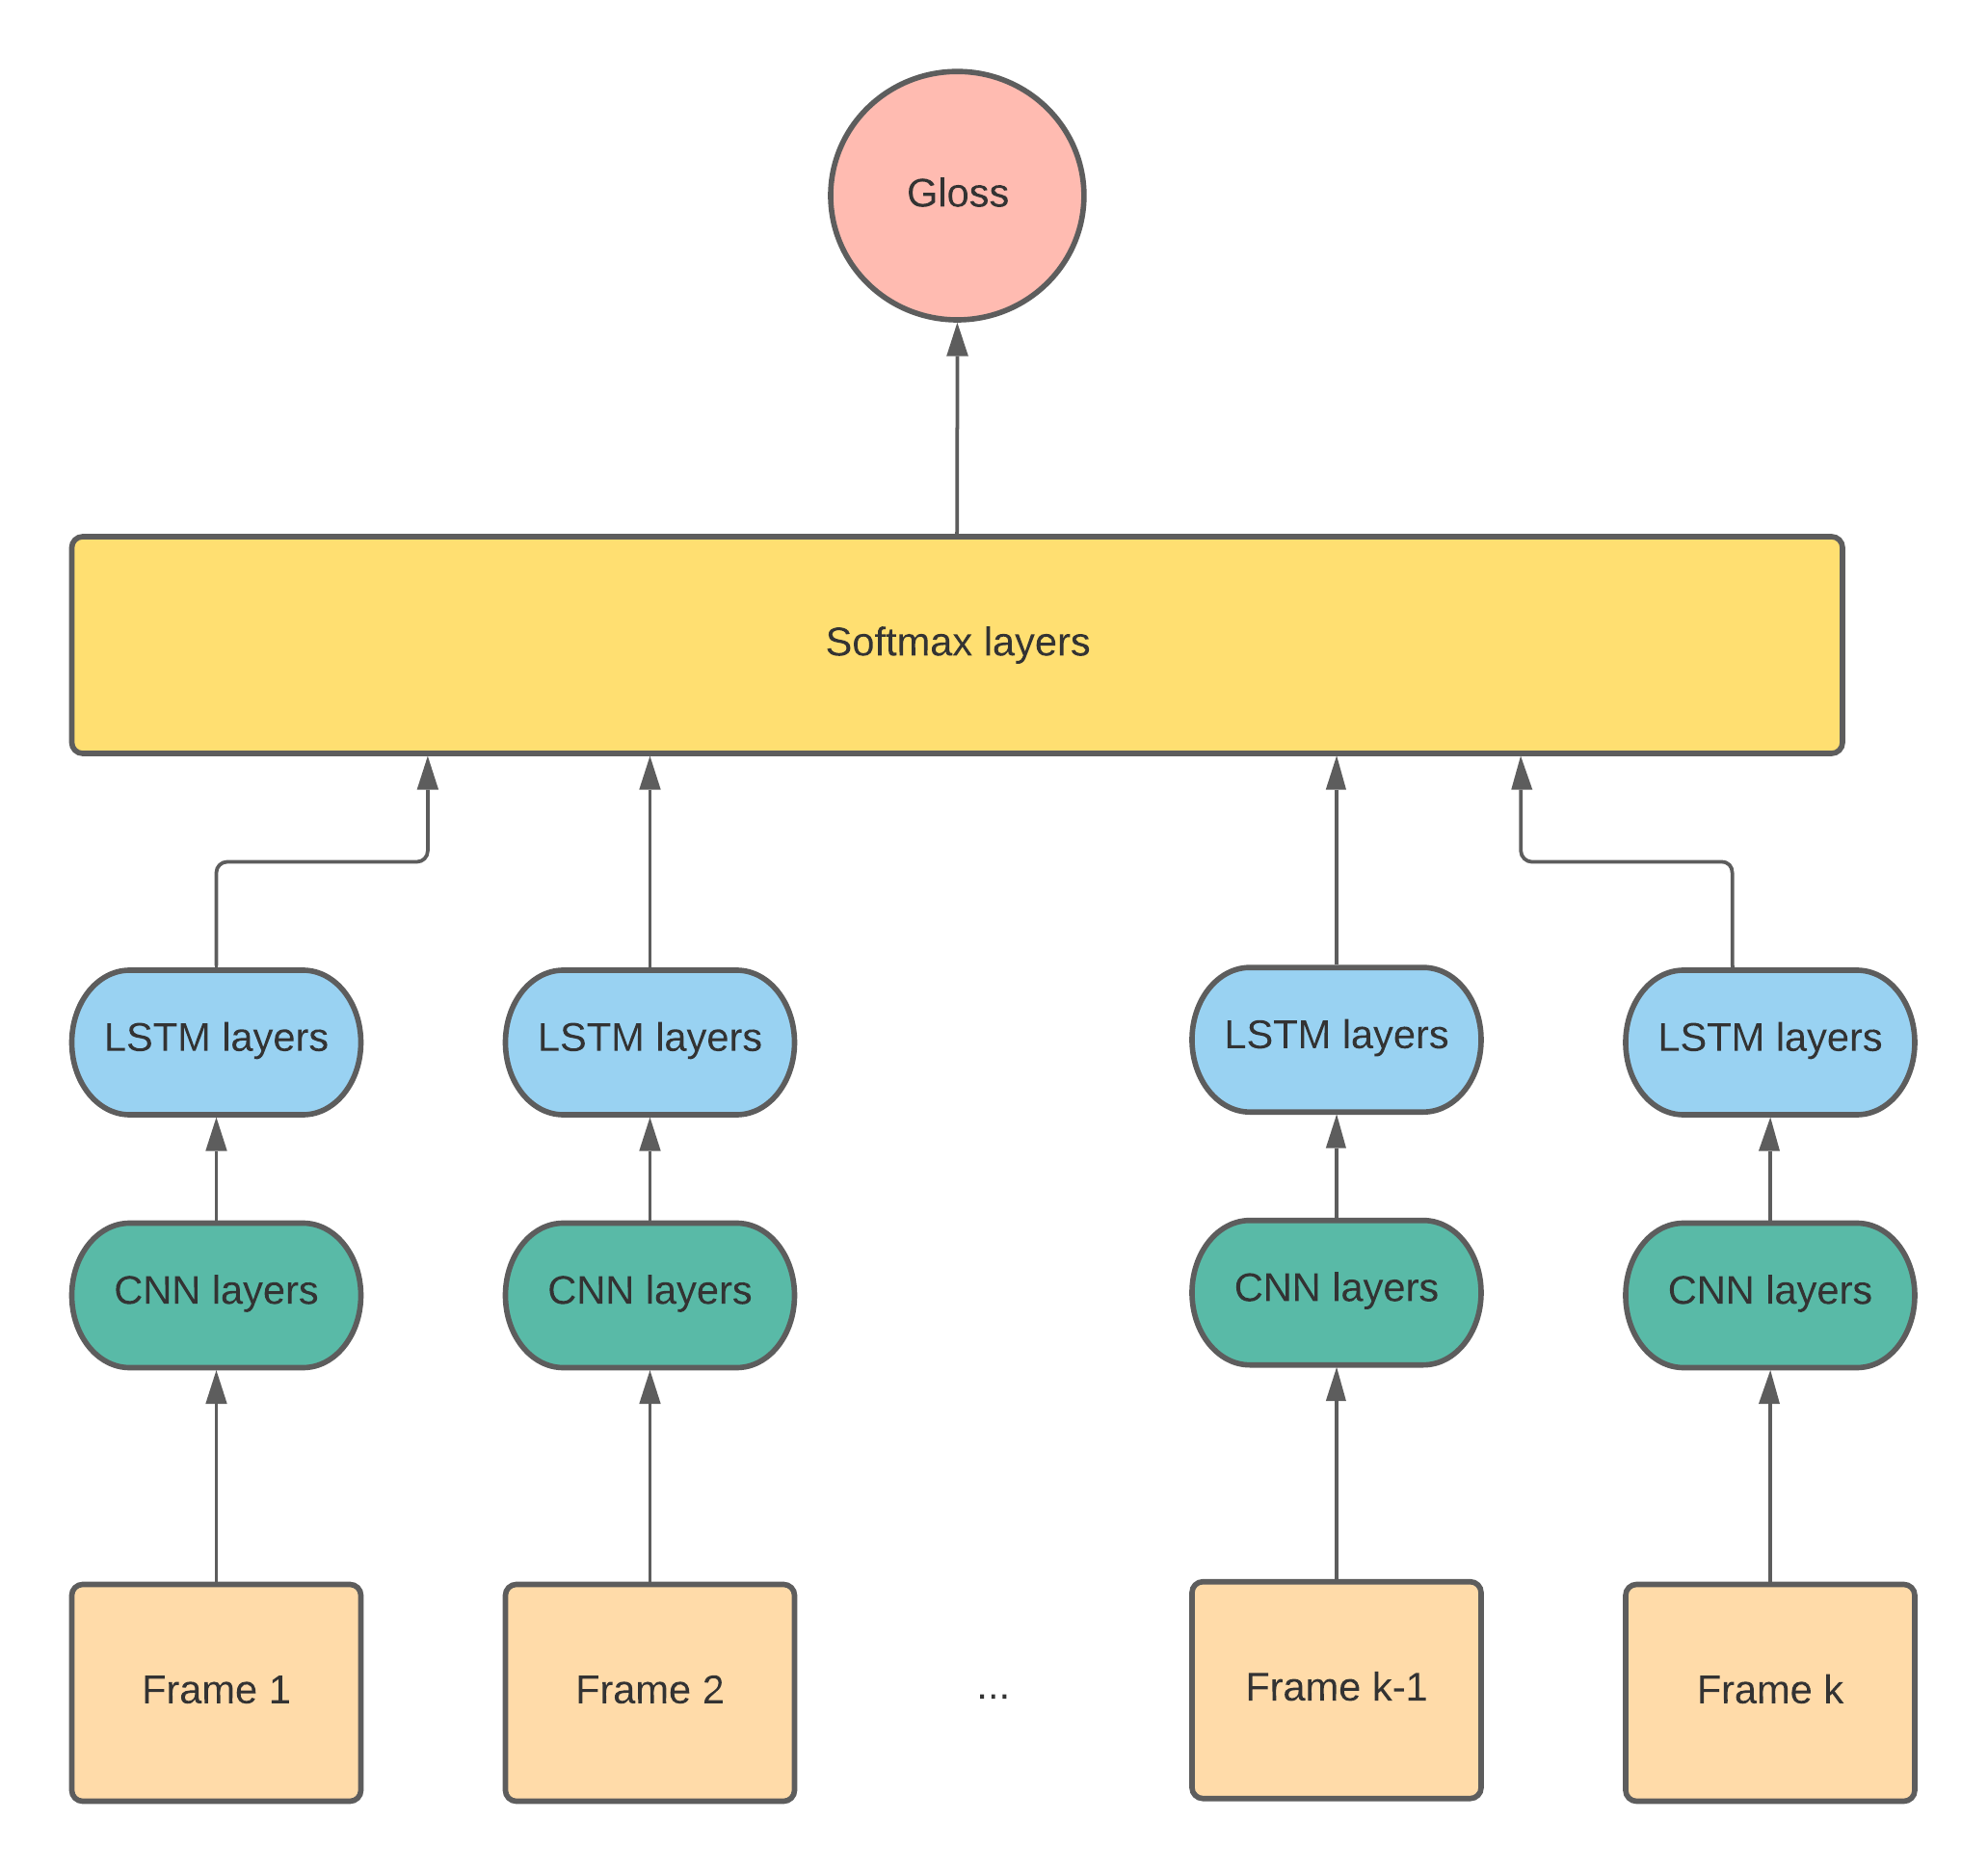
\includegraphics[width=0.75\textwidth]{CNN-LSTM.png}
    \caption{CNN-LSTM model}
    \label{Figure CNN-LSTM}
\end{figure}

In the model of ConvNet-LSTM, features are extracted separately from each frame of a video through a CNN network \citep{karpathy2014large}. Then they are feeded into a LSTM layer \citep{yue2015beyond,donahue2015long}, which is capable of providing stage encoding and temporal ordering. Finally, a fully connected layer is put on the top for classifer.

\subsubsection{3D ConvNet}
Extended from 2D ConvNet, in which convolutions exclusively generate features based on spatial dimensions, 3D ConvNet computes features in the spatial as well as temporal dimensions. Convolution using a 3D kernel is done by convolving a cube of several frames to get a 3D result. This architecture has the additional advantage of making the feature maps in the convolution layer linked to several contiguous frames in the preceding layer, which aids in the capture of motion information \citep{Ji20133DCN}. The use of 3dConvNet have been exploited in many researchs \citep{tran2015learning,taylor2010convolutional}. 

With \textit{\begin{math} c \times l \times h \times w \end{math}} size of a video (c is a number of channel, l is a number of frames, h and w are corresponding to height and width of each frame),
kernel size for 3D convolution and pooling are denoted by the notation \textit{\begin{math}d \times k \times k\end{math}}, where \textit{d} is the kernel temporal depth and \textit{k} is kernel spatial size, 3D ConvNet networks are programmed to accept video clips as inputs and predict the class label that correlate to \textit{n} classes based on datasets \citep{tran2015learning}.

\begin{figure}[H]
    \centering
    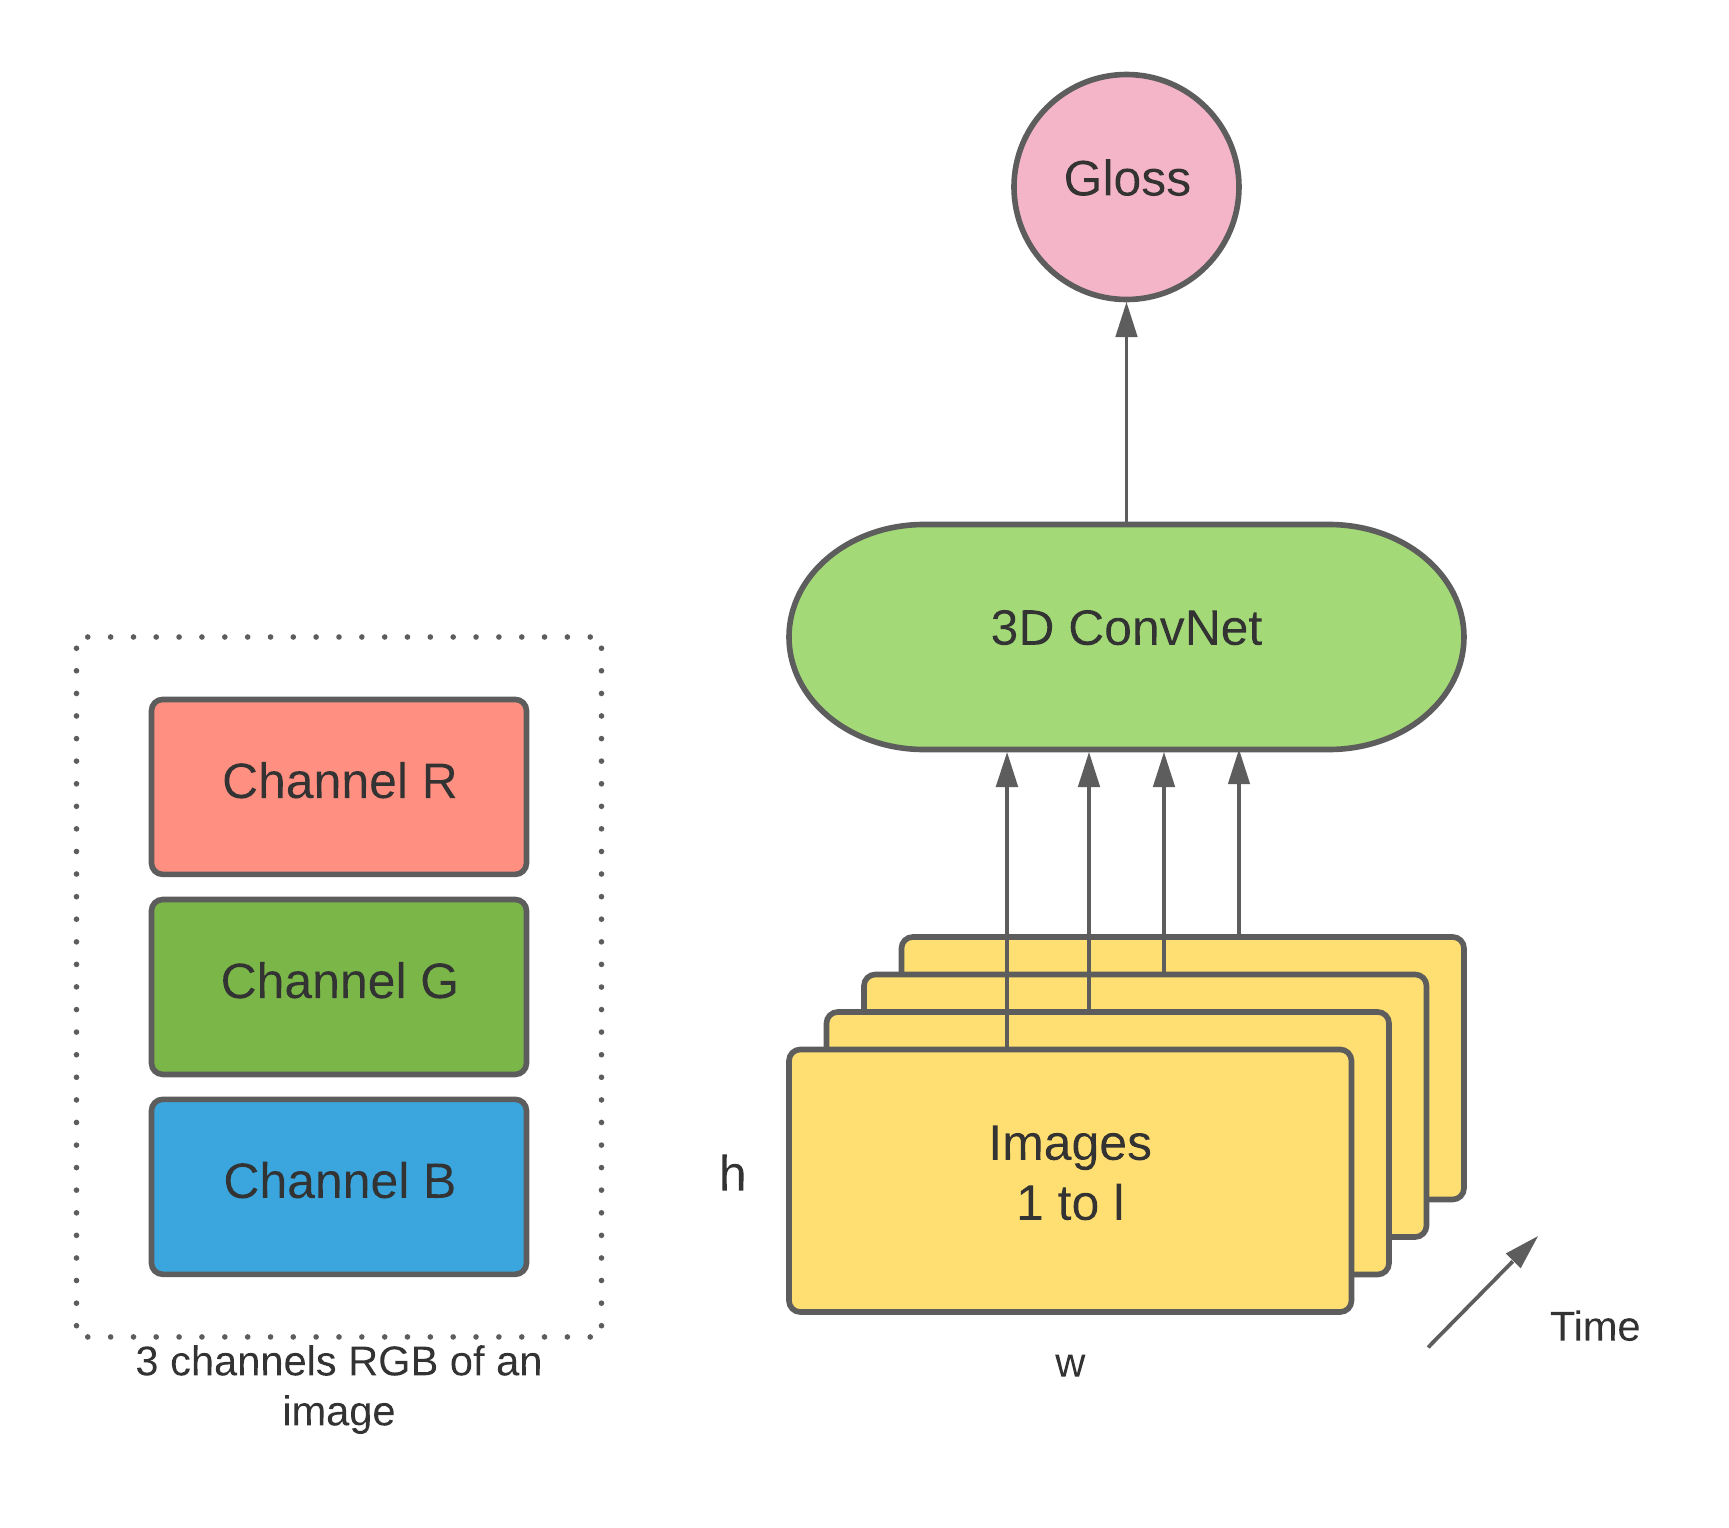
\includegraphics[width=0.75\textwidth]{3D ConvNet Model.png}
    \caption{An example of 3D ConvNet with RGB video as input}
    \label{Figure 3D ConvNet}
\end{figure}

\subsubsection{Two-stream network}
Introduced by Simonyan and Zisserman et al, a model which uses an individual RGB frame and an external n-frame optical flow, was shown extremely high performance on benchmarks, while also being efficient to train and test \citep{simonyan2014two}. In details, a video data is separeted into two streams, spatial stream and temporal stream. The spatial stream can spot motion in static frames, whereas the temporal stream is trained to perceive motion in images as optical flows, both of them are developed with ConvNet \citep{simonyan2014two}.

\begin{figure}[H]
    \centering
    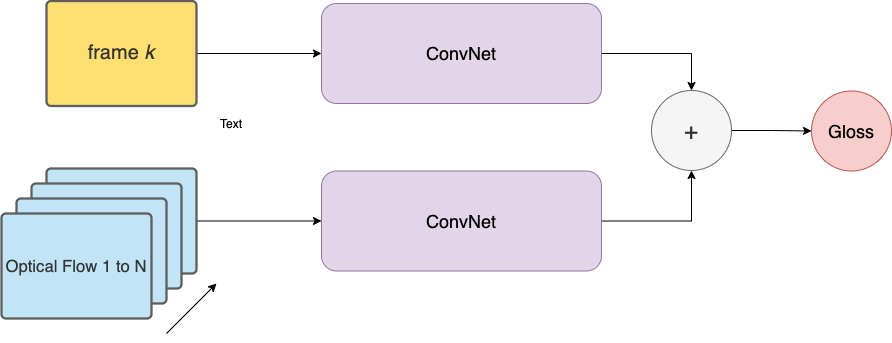
\includegraphics[width=0.75\textwidth]{Two-stream ConvNet Model.png}
    \caption{Two-stream 3D ConvNet model}
    \label{Figure 2-stream 3D ConvNet}
\end{figure}

The result shown by Simonyan and Zisserman indicates that using optical flow for training a temporal dimension is outperform than training on static frames \citep{karpathy2014large}.

An extended version of two-stream network, 3D-Fused Two-Stream, is using a 3D ConvNet which can learn patterns related to temporal directly \citep{carreira2017quo}. The model of 3d-Fused Two-Stream is as Figure 6.

\begin{figure}[H]
    \centering
    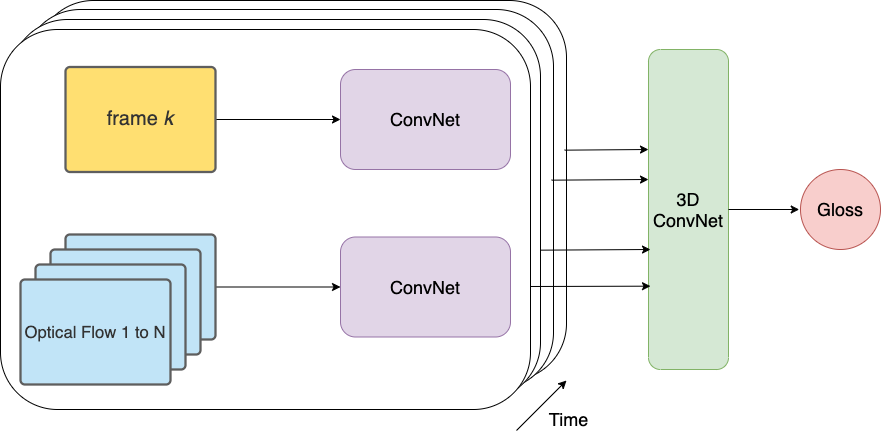
\includegraphics[width=0.75\textwidth]{3D-Fused Two-stream.png}
    \caption{3D-Fused Two-Stream}
    \label{Figure 3D-Fused Two Stream}
\end{figure}

\subsection{Model in this study}
With the extendable 2D ConvNet to 3D ConvNet where time dimensions can be added to perform the result, a coming up model is that use two streams of raw images and also optical flow frames. Thus, the temporal patterns is not only studied during the optical flow but also with RGB inputs. As a result, the performance is improved significantly compared with using only RGB stream \citep{carreira2017quo}.

In the method that Zisserman and Carreira proposed, 2 streams are trained independently, Therefore, with an input video, each stream will provide a prediction according to RGB frames and optical flow frames of it which are fed into two different I3D networks. Then next step is that the predictions of RGB stream and Optical Flow stream are computed averaged to give a final prediction.

\begin{figure}[H]
    \centering
    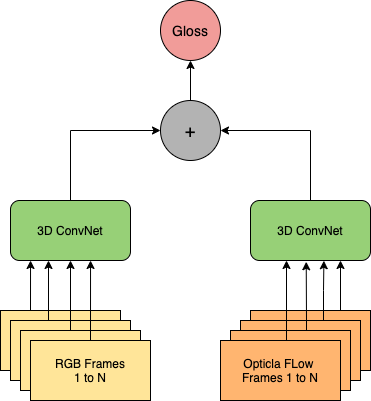
\includegraphics[width=0.7\textwidth]{2-stream I3D Model.png}
    \caption{2-stream 3D ConvNet by Zisserman and Carreira \citep{carreira2017quo}}
    \label{Figure 2-Stream 3D ConvNet}
\end{figure}

 The result of combining the predictions from RGB stream and optical flow stream is better that the prediction of each stream separately and also better than the results from other models \citep{carreira2017quo}. In the study, the group of author examined on several datasets for human recognition, such as UCF-101, HMDB-51, Kinitecs, the comparision if shown as the table below.

\begin{table}[H]
    \centering
    \resizebox{\textwidth}{!}{%
        \begin{tabular}{|c|c|c|c|c|c|c|c|c|c|}
        \hline
            \multirow{2}{*}{Architecture} & \multicolumn{3}{c|}{UCF-101} & \multicolumn{3}{c|}{HMDB-51} & \multicolumn{3}{c|}{Kinetics} \\ 
            \cline{2-10} 
            & RGB & Flow & RGB + Flow & RGB & Flow & RGB + Flow & RGB & Flow & RGB + Flow \\ 
        \hline LSTM & 81.1 & - & - & 36.0 & - & - & 63.3 & - & - \\ 
        \hline 3D ConvNet & 51.6 & - & - & 24.3 & - & - & 56.1 & - & - \\ 
        \hline 2-Stream & 83.6 & 85.6 & 91.2 & 43.2 & 56.3 & 58.3 & 62.2 & 52.4 & 65.6 \\
        \hline 3D-Fused & 83.2 & 85.8 & 89.3 & 49.2 & 55.5 & 56.8 & - & - & 67.2 \\ 
        \hline 2-Stream I3D & 84.5 & 90.6 & 93.4 & 49.8 & 61.9 & 66.4 & 71.1 & 63.4 & 74.2 \\ \hline
        \end{tabular}%
    }
    \caption{Comparision betwen models on several human activity datasets \citep{carreira2017quo}}
    \label{table comparision result of models}
\end{table}

With an amazing result compared to others, this study use the architecture of 2-stream I3D network to see how good it is when apply to recognize sign languages instead of human activies.

\section{Convolution Neural Network in image classification}
\subsection{Introduction of CNNs}
The heart of Deep Learning algorithms rely on Artificial Neural Networks (ANNs) what immitate the behaviors of human braind in which signals are send between neurons \citep{ibmANN}. Various neural network types are employed for certain use cases and data types and CNNs is a specific netwwork which are primarily focus to solve the problem of classification and computer vision tasks. Before the use of CNNs, to identify an object in images, feature extraction approaches were applied, however it were time-consuming and manual methods. With the introduction of convolutional neural networks, a more scalable technique to image classification and object identification has been made available. This methodology, which leverages linear algebra concepts, relies on matrix multiplication to find patterns inside an image. Most of CNNs have expensive computation, therefore to train model effectively, graphical processing units (GPUs) are required.

\begin{figure}[H]
    \centering
    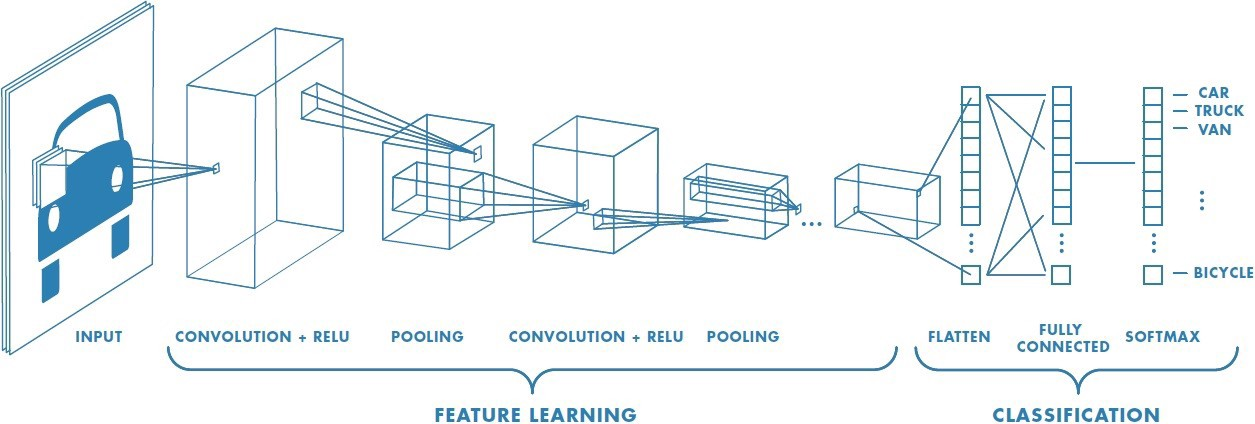
\includegraphics[width=0.8\textwidth]{Example of Classification by using CNN.jpeg}
    \caption{Example of CNN for classification}
    \label{Figure CNN for classification}
\end{figure}

A key difference between convolutional neural networks and other neural networks is their strength ability to handle voice, audio or image inputs. In the architecture of CNNs, there are 3 primary types of layers:  convolutional layers, pooling layers and fully connected layers \citep{ibmConvNet}.
\subsubsection{Convolution layer - the kernel}
The convolutional layer is the fundamental building element of a CNN, where most of computation occurs. The main component of convolution layers are input data, a filter and feature mapping. For instance, an image can be consider as a matrix of \textit{$width \times high \times channel$}, a video is matrix of \textit{$width \times high \times channel \times times$}. Then a kernel or filter, named as feature detector, will evaluate for the presence of a specific feature by moving across the fields of images. The final output of this processing is called as an activation map, feature map or convoluted feature \citep{dumoulin2016guide}.

\begin{figure}[H]
    \begin{subfigure}[b]{0.5\textwidth}
        \centering
        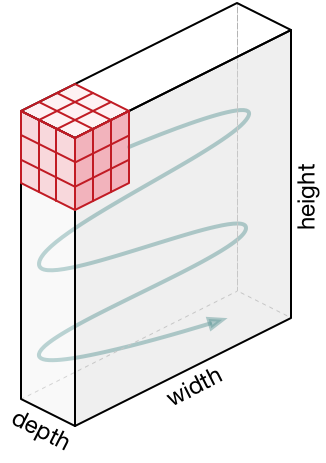
\includegraphics[width=0.5\textwidth]{Movement of Kernel.png}
        \caption{Kernel Movement}
    \end{subfigure}
    \hfill
    \begin{subfigure}[b]{0.5\textwidth}
        \centering
        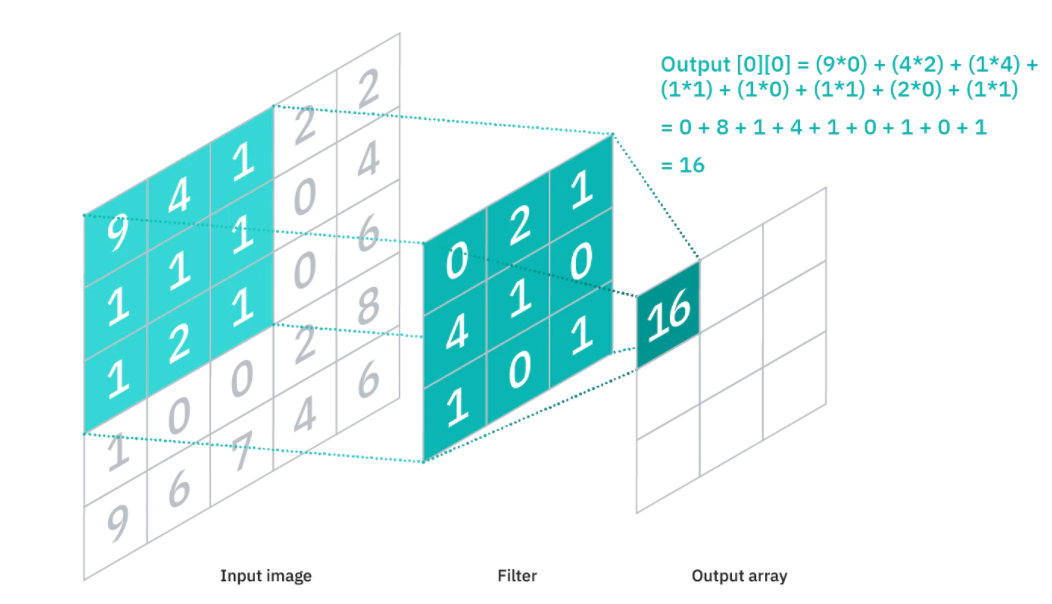
\includegraphics[width=0.8\textwidth]{Convolution process.png}
        \caption{Convolution Processing}
        \label{Convolution process}
    \end{subfigure}
    \hfill
    \caption{Kernel movement and Convolution Processing}
    \label{Figure CNN kernel and process}
\end{figure}

A kernel is a matrix of weights and the dimensions of the kernel is as same as the dimensions of input parameter of a convolutional layer, for example, with 2D convolutions, 2D matrix is used as kernel matrix. On the other hand, the filter is set of kernels, and each kernel is applied to a specific channel. Therefore, a filter have one more dimension compared to the dimension of kernel. If size of kernel is $h \times w$, and with k channels, filter's dimension is $k \times h \times w$ \citep{albawi2017understanding}. Through the convolution operation, the high-level feature such as edges are extracted. Convolutional layer is not restricted to only one. Normally, the first layer of convulutional captures low-level features such as color, gradient orientation, edges. Adding more layers allows the architecture to be able to adapt high-level characteristics which gives us a network that fully understanding image in the dataset.

However, there are problems with convolutions to be considered. As the example in \ref*{Convolution process}, with the $5 \times 5$ matrix input, after applying the filter, the size of output matrix is $3 \times 3$. Thus, the image size is shrinked every convolution operation. Because of multi convolutional layers in the network, the original image gets smaller; however it is not expected to be shrinked every time \citep{szegedy2015going}. Another matter is that every time the kernel moves accross the images, the edges of objects inside the picture have less number of touches than the middle area of the objects, and the middle areas are also overlapped. So the output does not reflect much about the information of corner features and edges in an image. Padding is a solution to tackle these issues by keep the size of the images preserve.

\begin{figure}[H]
    \centering
    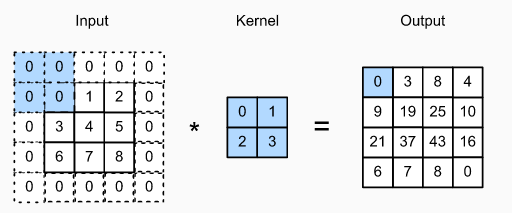
\includegraphics[width=\textwidth]{padding.png}
    \caption{Example of padding}
    \label{Padding}
\end{figure}

So if the input matrix has size $n \times n$, filter matrix is $f \times f$ with the padding p, then the matrix output will have the size of $(n + 2p - f + 1) \times (n + 2p -f + 1)$. In the exxample in \ref{Padding}, p is 1 while orginal input size is $3 \times 3$ and $2 \times 2$ is the size of filter matrix.

Another hyperparameter related to convolution neural networks is stride. As definition, stride is number of pixels that filer matrix moves each step across the horizontal or vertical  position. The size of convolution output is depened on padding and stride hyperparameters. With padding p, $f \times f$ filter matrix, $n \times n$ input matrix, and stride s, the output dimension will be $[{(n + 2p - f + 1) / s } + 1] \times [{(n + 2p - f + 1) / s } + 1]$

\begin{figure}[H]
    \centering
    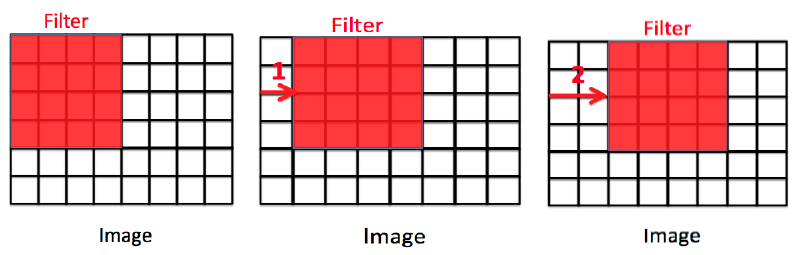
\includegraphics[width=\textwidth]{stride.png}
    \caption{Example of stride = 0, 1, 2 respectively.}
\end{figure}

\subsubsection{Pooling layer}
Besides convolution computations, pooling operations is responsible to build up essential blocks in CNNs by decreasing the spatial size of convovled feature, or reducing the number of parameter input \citep{dumoulin2016guide}. By this, computational power required also decrease because of dimensionality reduction. Additionally, it is beneficial for extracting dominant features which are positional and rotational invariant, thus allows the model to properly trained. The pooling operation works similarly as the convolutional layer in that it sweeps a filter across the input, except that the filter does not contain any weights \citep{albawi2017understanding}. There are two types of pooling \citep{ibmConvNet}:

\begin{itemize}
    \item Max Pooling: with each pass of the filter over the input, the highest value is selected to the output array. This technique is more commonly implemented compared with avarage pooling.
    \item Average Pooling: instead of choosing a max value of input, tt computes the average value inside the receptive field, then send to output array.
\end{itemize}

\begin{figure}[H]
    \centering
    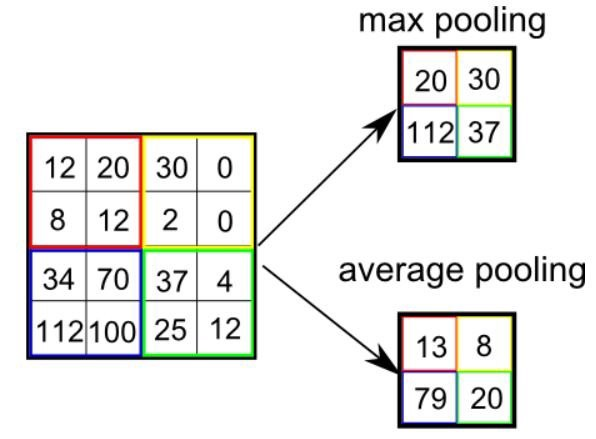
\includegraphics[width=0.6\textwidth]{Pooling.png}
    \caption{Pooling}
    \label{Figure Pooling}
\end{figure}

The pooling layer has a few drawbacks, but is also advantageous to the CNN. They simplify, optimize, and minimize the danger of overfitting.

\subsubsection{Fully Connected (FC) Layers - Classification}

\begin{figure}[H]
    \centering
    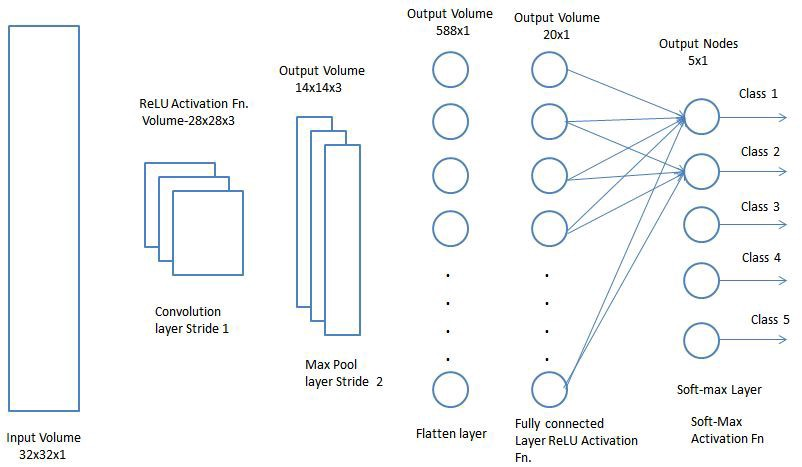
\includegraphics[width=0.7\textwidth]{Fully connected.jpeg}
    \caption{Fully Connected layer \citep{towardScienceCnn}}
    \label{Figure FC layer}
\end{figure}

It is typically inexpensive to add a Fully Connected Layer after convolutional layers to learn non-linear combinations of the features represented as output. The name of the full-connected layer accurately reflects its characteristics. A good description of the layer is that each node in the output layer connects to all nodes of the previous layer \citep{8308186}. Using the characteristics gathered from the preceding layers and their various filters, this layer conducts the duty of categorization on the data. Contrary to convolutional and pooling layers, which often employ ReLu functions to categorize inputs properly, FC layers typically employ a softmax activation function to give results in a probability ranging from 0 to 1 \citep{ibmConvNet}

\subsection{1D, 2D, 3D Convolutions}
When it comes to time series data processing, 1D Convolutions are widely used because the input in such cases is one dimension. Mentioned previously, multi channels can stack with the 1D data input.
As the filter can travel in one direction only, then the output only have 1D.

\begin{figure}[H]
    \centering
    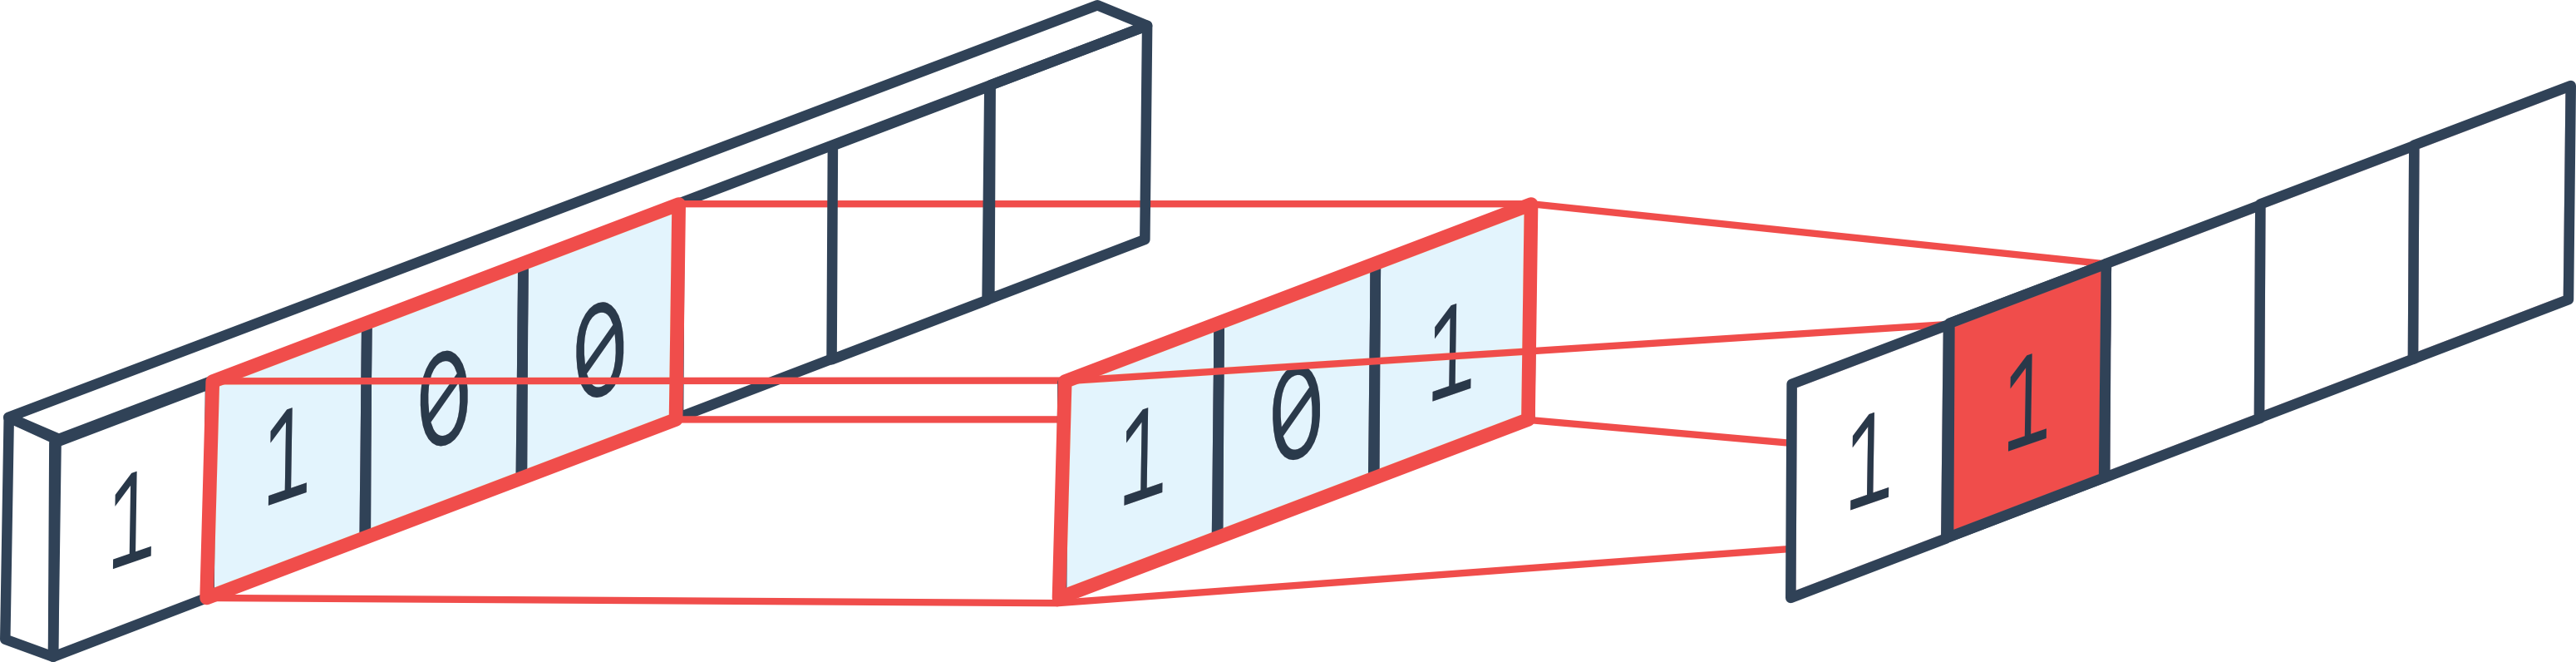
\includegraphics[width=0.5\textwidth]{1D Conv.png}
    \caption{1D Convolution}
    \label{Figure 1D}
\end{figure}

The diagram below visualize how 2D convolutions is. As mentioned before, 2D data also have multiple channels, so the filter can move in 2 directions and lead to the final 2D output. In computer vison, 2D convolutions are the most common convolutions. In case of 3D convolutions, it is hard to visualize the filter because of 4 dimensions the filter has, so only the 3D convolutions with single channels is visualized as the figure below. Like others, in 3D convolutions, the filter can move in 3 directions therefore the output is 3 dimentions.

\begin{figure}[H]
    \begin{subfigure}[b]{0.4\textwidth}
        \centering
        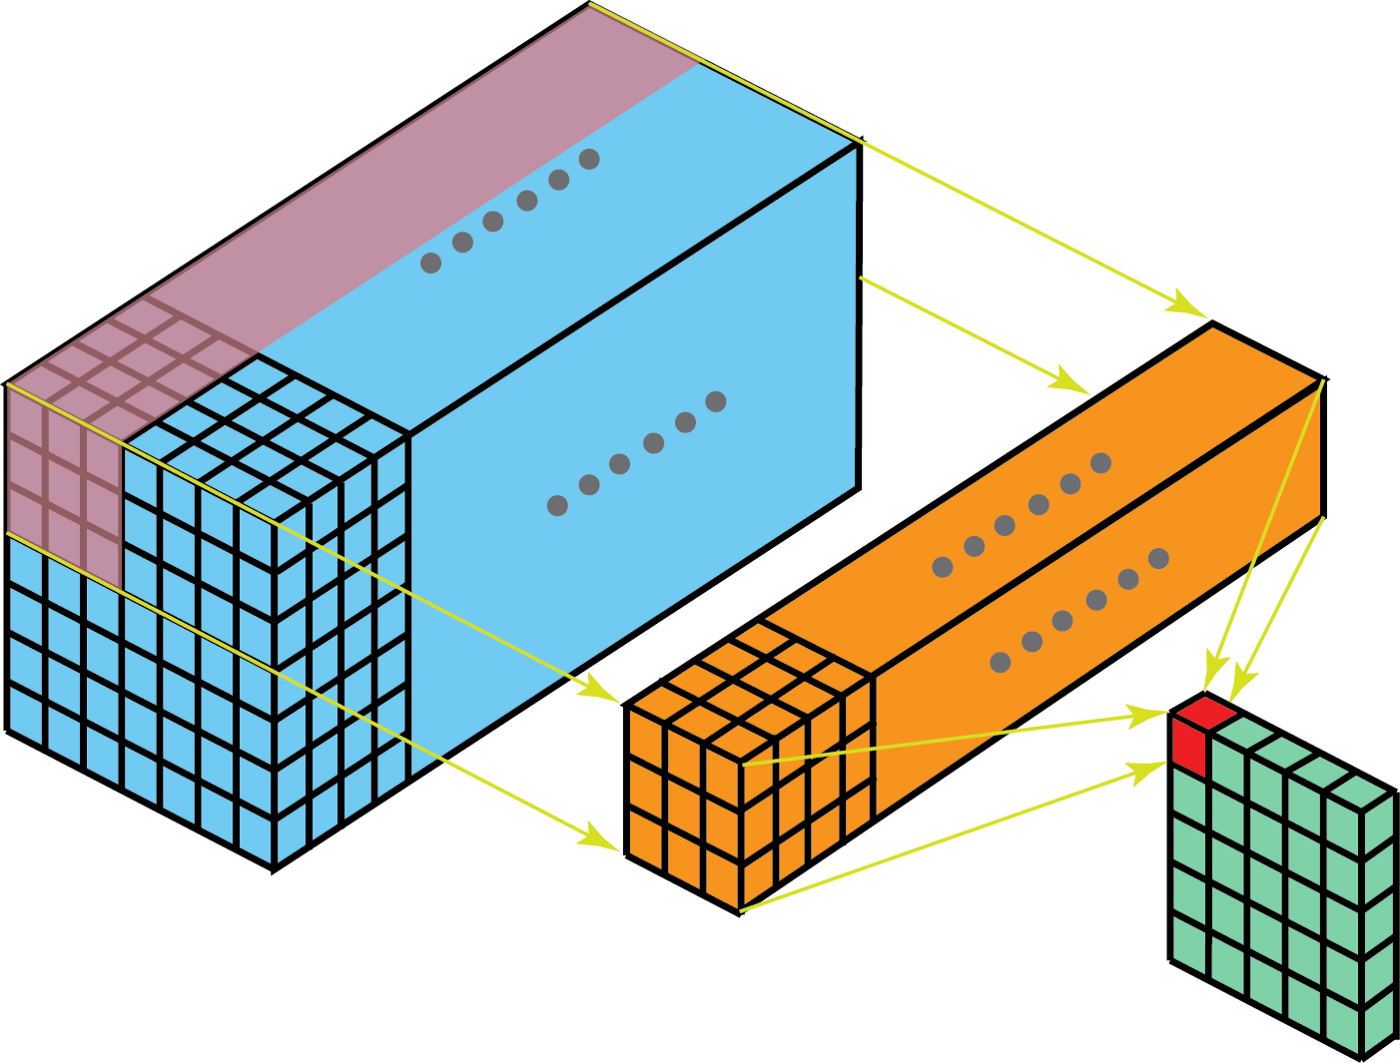
\includegraphics[width=0.8\textwidth]{2D Conv.png}
        \caption{2D Convolutions}
        \label{a}
    \end{subfigure}
    \hfill
    \begin{subfigure}[b]{0.6\textwidth}
        \centering
        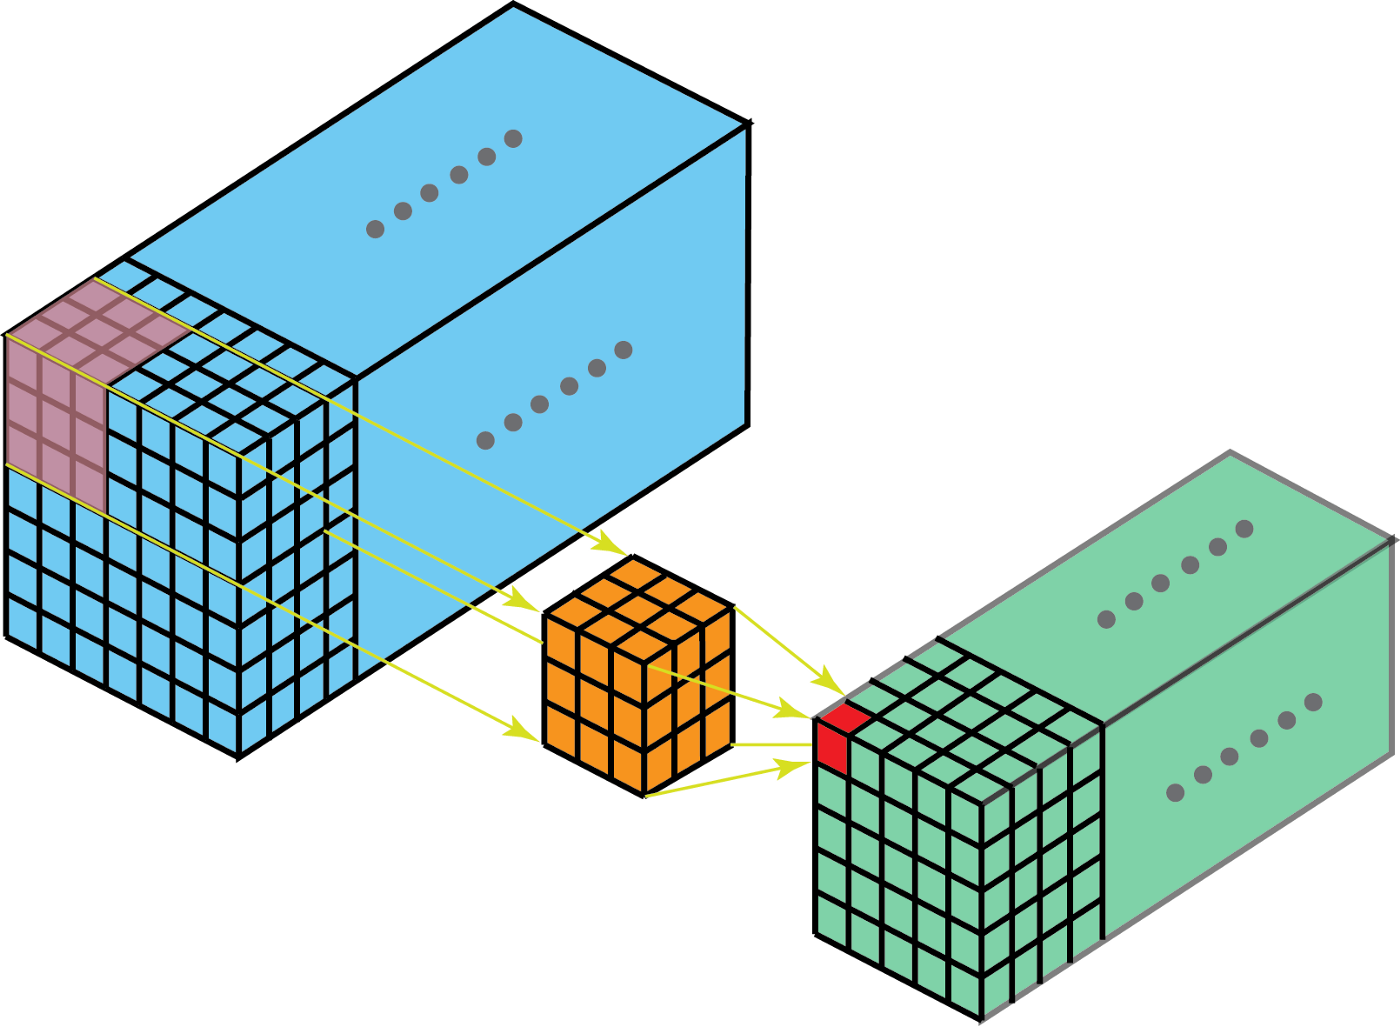
\includegraphics[width=0.6\textwidth]{3D - single channel.png}
        \caption{3D Convolutions with single channel}
        \label{b}
    \end{subfigure}
    \hfill
    \caption{2D and 3D Convolutions}
    \label{Figure 2D 3D}
\end{figure}

\section{Techniques for Inflated 3D ConvNet}
\subsection{Inflating 2D ConvNets into 3D ConvNets}
In order to prevent spending to much time in the process of training spatio-temporal models, a simply approach is applied to utilize the successful of 2D (image) classification architectures into 3D ConvNet when 2D classified models have been achieved many significant improvements in years. As a result, the filters and pooling kernels that are coming from the 2D architectures are inflated with one more dimension, temporal dimension. So that they are from a $N \times\ N$ matrix to a $N \times N \times N$ cubic \citep{carreira2017quo}.

\subsection{2D filters to 3D filters}
In additional, the input parameters can also be boostrapted by adopting pre-trained ImageNet models. As can be seen, a video (boring video \citep{carreira2017quo}) can be made from an individual image by cloning the image many times into video scenes. Thus following the linearity, 2D filters weights are repeated N times according to time dimension and then rescaling by dividing by N. In this way, 3D ConvNet models can be implicitly train on Imagenet in which the pooled activation of boring video are the same with the input of single image. It means that the computation outputs of non-linearity layers, max and average pooling layers are as same as the 2D case \citep{mansimov2015initialization}.

\subsection{Receptive field}
To comparing with 2D models, another change to take into account is the receptive field of pooling and convolutional layers. As described before, an input vector for a convolutional neural network is an area of an image which is accessible to a filter per time and as more layers it is more increasing. 2D convolutions and pooling are symmetrical because they concentrate on image width and height (for example 7x7 kernel is accetable because it is symmetrical while a kernel 7x5 is not). When the temporal dimension is taken into consideration, it is necessary to determine the optimum receptive field, which is dependent on the frame rate and the picture dimensions of the image. \citep{towardScienceI3DUnderstanding}. According to Zisserman and Carreira, the problem of symmetric receptive field is that if it develops too rapidly in time compared to space, it may confuse edges from different objects, leading to poor feature detection; on the other hand, if it grows too slowly, dinamically scence might be fail to be captured \citep{carreira2017quo}. In the final, I3D kernels are not symmetrical due to the inclusion of temporal dimension.

\subsection{Network Architecture}
The network diagram is as the figure below \cite{carreira2017quo}

\begin{figure}[H]
    \centering
    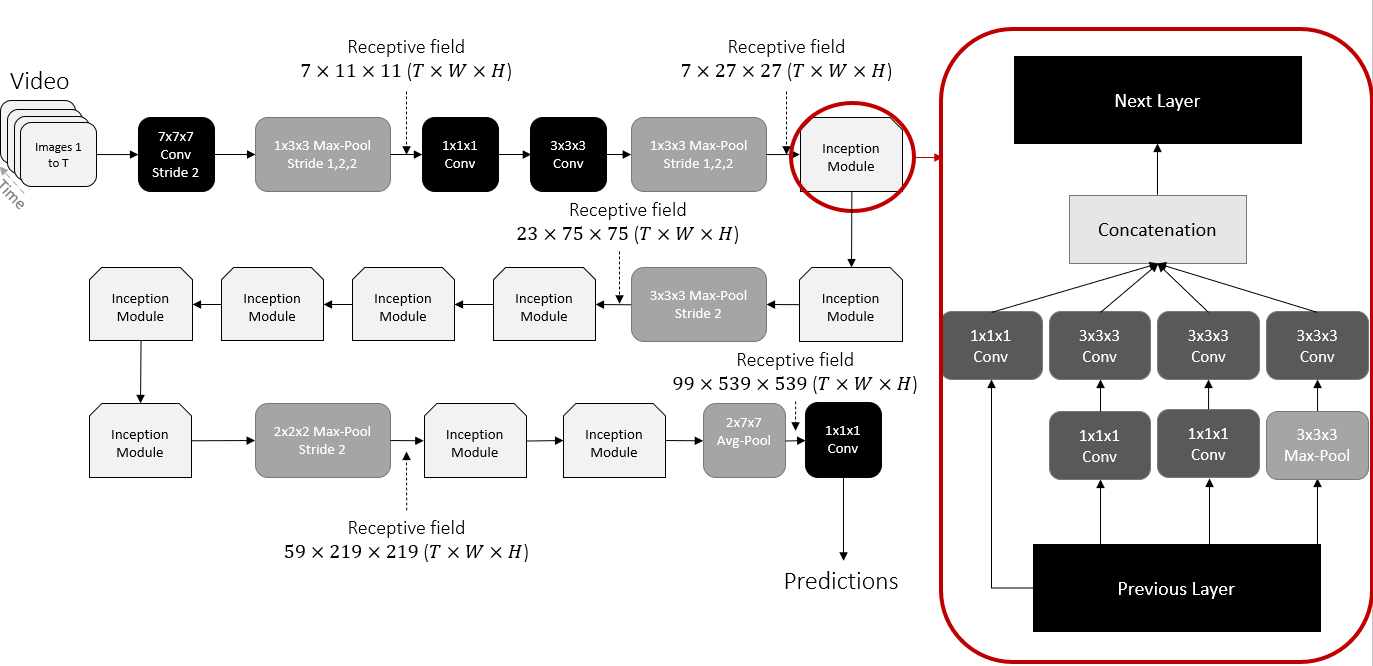
\includegraphics[width=\textwidth]{Stream architecture.png}
    \caption{Network architect \citep{carreira2017quo}}
    \label{Figure}
\end{figure}

To be seen in the diagram, as the begining an asymmetrical filters is used for max-pooling, keep time retains while doing pooled operations over image width and height dimensions. So far, the convolutions and pooling which related to time dimension are performed in the later stage. In this paper, the Inception module is not described in details, however it is used widely in 2D classification networks. The Inception module aggregates the results after evaluating spatial (and time in case of classifying video) information at multiple scales. In the proposal of Inception model, after going through the $1 \times 1 \times 1$ convolution, the number of input channels is reduced before passing into the larger convolution $3 \times 3 \times 3$, so the computations are less expensive compared to the alternative.

\section{Optical flow}
\subsection{Introduction}
Optical flow is a representation of the mobility of a scene environment in relation to an observer's position. In the problem of recognizing human gesture, a static scence in a single frame can lead to an ambiguity in interpreting gesture class.  The movement of human bodies must be taken advantage of in order to have a thorough grasp of the gesture class. There are a variety methods for calculation optical flow from frame to frame, including region-based, energy-based, differential-based, phase-based \citep{marco2018computer}. The differential technique is the most frequently used method, and it is based on the premise of picture brightness constancy \citep{horn1981determining}.

\begin{figure}[H]
    \centering
    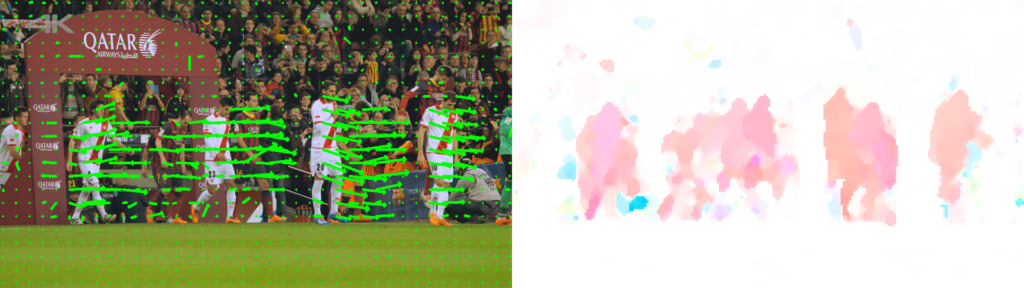
\includegraphics[width=\textwidth]{Football-1024x288.png}
    \caption{Example of an optical flow frame \citep{opticalflowExample}}
    \label{Figure x}
\end{figure}

Assume that the constant brightness of a pixel \textit{(x, y)} in an object does not change; it is not true in reality, however it is reasonable and natural when the time is small enough. Therefore, the image intensity of two continuous frames can expressed by the equation below \citep{o2005optical}.

\begin{equation} \label{eq1}
    I(x, y, t) = I(x +\delta x, y + \delta y, t + \delta t)
\end{equation}
\myequations{Constant intensity assumption}

Then, using Tayloy Series Approximation of the RHS:

\begin{equation} \label{eq2}
    I(x, y, t) = I(x, y, t) + \frac{\partial I}{\partial x}\delta x + \frac{\partial I}{\partial y}\delta y + \frac{\partial I}{\partial t}\delta t
    \\
    \Rightarrow \frac{\partial I}{\partial y}\delta y + \frac{\partial I}{\partial t}\delta t = 0
\end{equation}
\myequations{Taylor Series Approximation of pixel intensity}

Next, \textit{d}t is divided to derive optical flow equation

\begin{equation} \label{Op Flow equa}
    \frac{\partial I}{\partial x}u + \frac{\partial I}{\partial y}v + \frac{\partial I}{\partial t} = 0
\end{equation}
\myequations{Optical flow equation}

Noted that $u = \frac{\textit{d}x}{\textit{d}t} $, $v = \frac{\textit{d}y}{\textit{d}t} $ and $\frac{\textit{d}I}{\textit{d}x} $, $\frac{\textit{d}I}{\textit{d}y} $, $\frac{\textit{d}I}{\textit{d}t} $ can be considered as the image gradients along to horizontal, vertical and time dimensions. So far, optical flow problem is that sovling $u(\frac{\textit{d}x}{\textit{d}t})$ and $v(\frac{\textit{d}x}{\textit{d}t})$ \citep{o2005optical}. However, the issue could not be solved with only one equation with two unknow variables.

There are two type of optical flow: Sparse and Dense optical. In details, Sparse optical flow requires a pre-processing step in which some \textit{"interesting features"} (pixels of object's edges or corners) are detected and then only calculate flow vectors of those pixels \citep{chuanenMotionEstOpticalFlow}. On the other hand, computation cost for Dense Optical Flow is expensive and slow performance \citep{wulff2017optical} because it provides flow vectors of entire frames, one flow vector per pixel.

\subsection{Algorithm for converting RGB video into Optical Flow video}
\subsubsection{Lucas-Kanade: Sparse Optical Flow}
As mentioned above, the initial step of calculating Sparse optical flow is extracting interesting features which are points in images and present rich content information \citep{harris1988combined}. They are made up of two main things:

\begin{itemize}
    \item \textbf{Interesting points:} The points which are immune when an image is rotated, translated, scaled or intensified. For instance, pixels which are related to edges, corners or blobs can be considered as interest points inside an image \citep{derpanis2004harris}.
    \item \textbf{Feature Descriptors:} These findings outline the patch of images near the interest points in vectors, from raw pixel to complex Histogram of Gradients (HoG) \citep{derpanis2004harris}.
\end{itemize}

One of a popular method for corner detection is Harris Corner Detector which was proposed in 1988 by Chris Harris and Mike Stephens in the paper "A combined Corner and Edge Detector". The idea of them is that determine the intensity difference for a movement of \textit{(u, v)} in all directions. It is expressed in the mathematic form as \citep{harris1988combined}:

\begin{equation} \label{eq3}
    E(u, v) = \sum_{x, y} \underbrace{w(x, y)}_\text{window function} [\underbrace{I(x + u, y + v)}_\text{shifted intensity} - \underbrace{I(x, y)}_\text{intensity}]^2
\end{equation}
\myequations{Weighted sum multiplied by the intensity difference for all pixels in a window}

\begin{figure}[H]
    \centering
    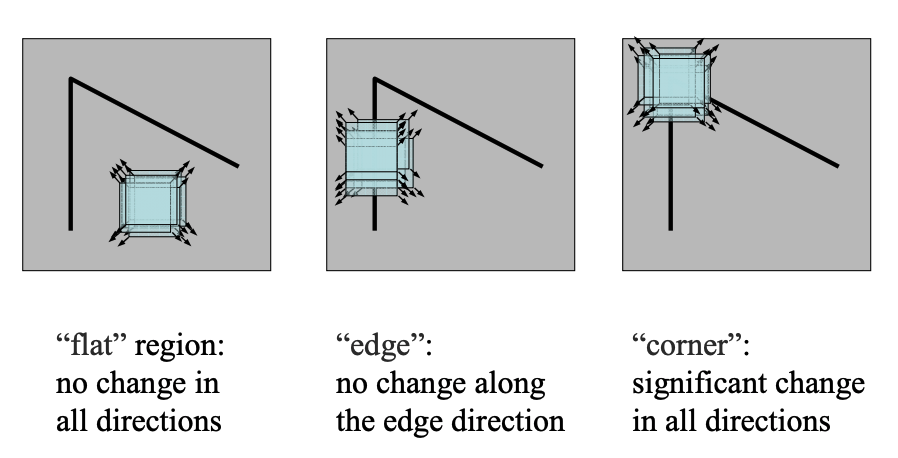
\includegraphics[width=0.7\textwidth]{Basic idea of Harris Corner Detector.png}
    \caption{Harris Corner Dector basic idea}
    \label{Figure X}
\end{figure}

The Harris Corner Detector includes three primary steps \citep{ryu2011formula}:

\begin{itemize}
    \item It identifies which windows (small picture patches) generate extremely significant changes in intensity when moved in both the X and Y axes (i.e. gradients).
    \item Compute a score R for each window found.
    \item Important corners are selected and marked by applying an threshold to the score.
\end{itemize}

Another algorithm for corner dectected is Shi-Tomasi Corner Detector which was presented by Jianbo Shi and Carlo Tomasi in 1994 \citep{shi1994good}. The algorithm mostly as same as Harris Corner Detector, however the R score is calculated differently which makes the result better. Furthermore, Shi-Tomasi focuses only in the top N corners therefore it might be beneficial in case that each and every corner do not want to be detected.

Deep into the calcultion of R score to identify the diffrence between HDC and SCD.

\begin{table}[ht!]
    \centering
    \def\arraystretch{1}%
    \caption{HDC vs SDC Scoring function}
    \resizebox{\textwidth}{!}{
        \begin{tabular}{|c|c|}
            \hline \textbf{Harris Corner Detector} & \textbf{Shi-Tomasi Corner Detector} \\
            \hline 
                \begin{tabular}{@{}c@{}}$R = det M - k(trace M)^2$ \\ $det M = \mu_1\mu_2$ \\ $trace M = \mu_1 + \mu_2$
                \end{tabular} & $R = min(\mu_1, \mu_2)$ \\
            \hline
        \end{tabular}
    }
    \label{table:1}
\end{table}

\begin{figure}[H]
    \centering
    \begin{subfigure}{0.4\textwidth}
        \centering
        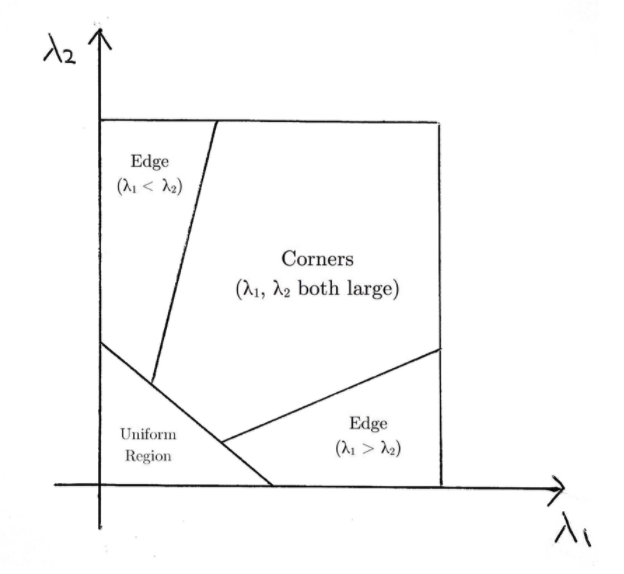
\includegraphics[width=\textwidth]{HDC R Scoring.png}
        \caption{Scoring function in HDC}
        \label{Scoring HDC}
    \end{subfigure}
    \begin{subfigure}{0.4\textwidth}
        \centering
        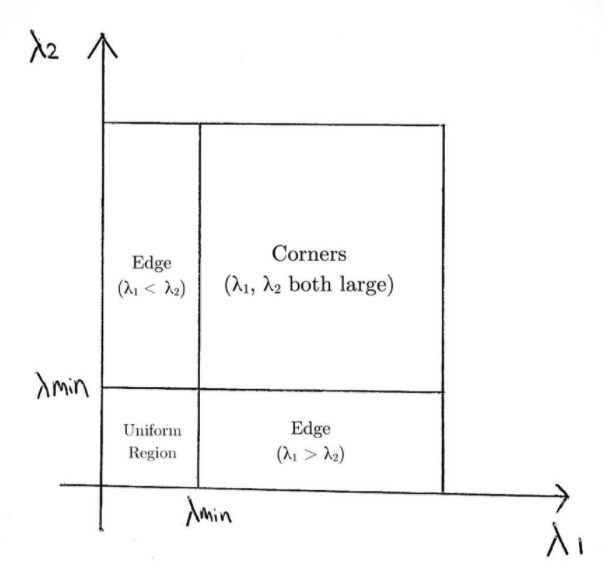
\includegraphics[width=\textwidth]{SDC R scoring.png}
        \caption{Scoring function in SDC}
        \label{Scoring SDC}
    \end{subfigure}
    \caption{Scoring function between HDC and SDC on $\mu_1$ - $\mu_2$ space}
    \label{Figure 10}
\end{figure}

The pictures below show the result of Harris and Shi-Tomasi Corner Detector.

\begin{figure}[H]
    \centering
    \begin{subfigure}{0.3\textwidth}
        \centering
        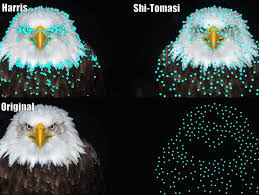
\includegraphics[width=0.8\textwidth]{HDC-SDC-1.jpeg}
    \end{subfigure}
    \begin{subfigure}{0.3\textwidth}
        \centering
        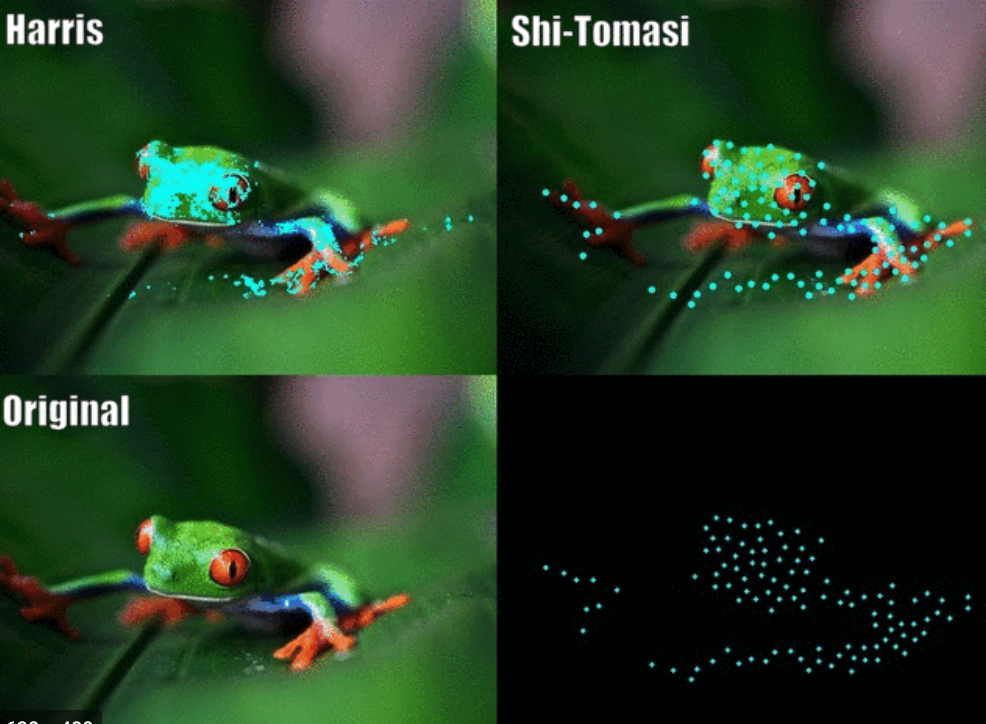
\includegraphics[width=0.8\textwidth]{HDC-SDC-2.png}
    \end{subfigure}
    \begin{subfigure}{0.3\textwidth}
        \centering
        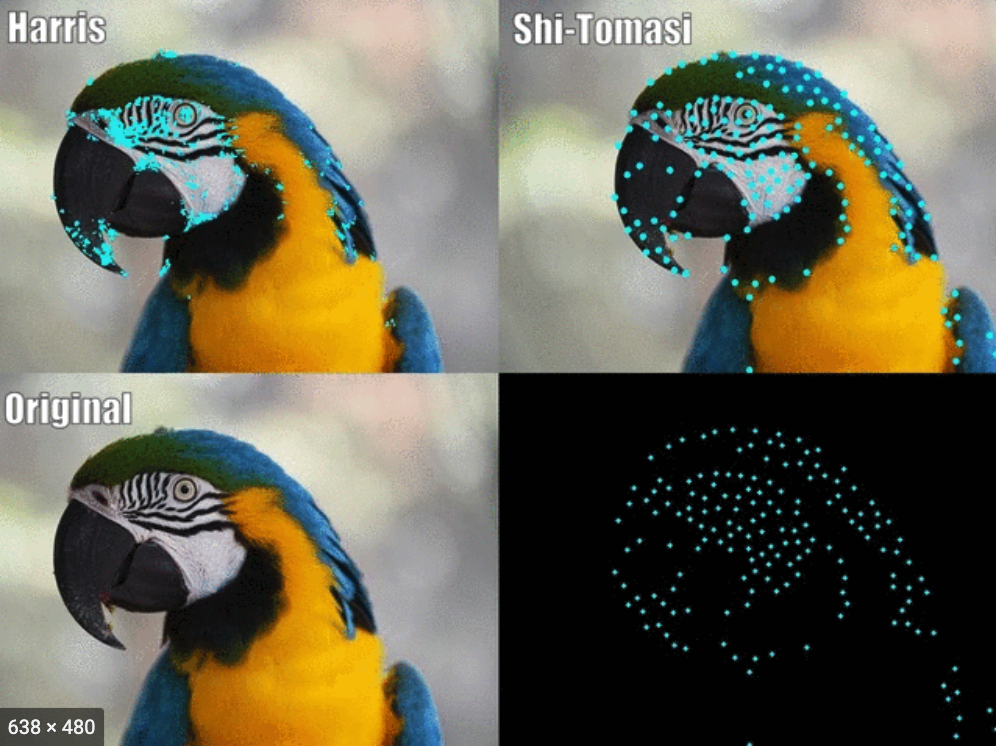
\includegraphics[width=0.8\textwidth]{HDC-SDC-3.png}
    \end{subfigure}
    \caption{Result of HDC and SDC algorithm for corner detection}
\end{figure}

Then based on an assumption that in the very small period ($\delta t$), the object is not moving much and objects in a frames is changed smoothly in shade of gray. So with this assumption, Lucas - Kanade proposed an idea that a small neighborhood $n \times n$ window arround features detected (by Shi-Tomashi detector) have the same motion. Therefore the partial derivates of image I respect to positon (x, y) and time t for a pixel q inside the window is described as equation \ref{pixel intensity equation}. It is Optical Flow Equation that described earlier.

The Lucas - Kanade algorithms can be implemented following:


\begin{equation} \label{pixel intensity equation}
    I_{x}(q_{n})V_{x} + I_{y}(q_{n})V_{y} = -I{t}(q_{n})
\end{equation}
\myequations{Optical Flow Equation - Lucas - Kanade algorithm}

Then in a form of matrix $Av = b$ where

\begin{center}
    $A = \begin{bmatrix}
        I_{x}(q_{n}) & I_{y}(q_{n})
    \end{bmatrix}$

    $v = \begin{bmatrix}
        v_{x} \\ v_{y}
    \end{bmatrix}$

    $b = \begin{bmatrix}
        -I_{t}(q_{n})
    \end{bmatrix}$
\end{center}
    
Now the issue is that solving two unknown variables $v_{x}$ and $v_{y}$ with n equations, so it is over-determined. To deal with this problem, least squares fitting is used as follow:

\begin{equation}
    \begin{bmatrix}
        v_{x} \\ v_{y}
    \end{bmatrix} = 
    \begin{bmatrix}
        \sum_{i}I_{x}(q_{i})^2 & \sum_{i}I_{x}(q_{i})I_{y}(q_{i}) \\
        \sum_{i}I_{y}(q_{i})I_{x}(q_{i} & \sum_{i}I_{y}(q_{i})^2
    \end{bmatrix}^{-1}
    \begin{bmatrix}
        -\sum_{i}I_{x}(q_{i})I_{t}(q_{i}) \\
        -\sum_{i}I_{y}(q_{i})I_{t}(q_{i})
    \end{bmatrix}
\end{equation}
\myequations{New optical flow equation: two-unknow-form equation}

Where $v_{x} = u = \frac{dx}{dt}$, $v_{y} = v = \frac{dy}{dt}$ indicate the movement of x and y over the time. The optical flow problem is completed when the two variable is sovled. So the algorithm identifies some key points and then calculate the optical flow vectors of these points. However, becauses of the assumption above, Lucas-Kaneda approach is only suitable for tracking object with slightly movements and not successful for large motion. Then the idea comes up compute optical flow from difference resolutions is offered with Open CV library. It is called pyramids method. In details, small motions can be ignored and the large motions are scaled to be small motions and then computed the optical flow based on the scaled motions.

\begin{figure}[H]
    \centering
    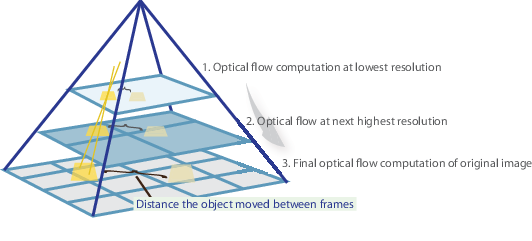
\includegraphics[width=\textwidth]{lucas-kanade-pyramid.png}
    \caption{Lucas - Kaneda pyramid method}
\end{figure}

Below pseudo-code show how to convert RGB frames into optical flow by using Lucas - Kanade algorithm with supported by OpenCV library.

\begin{algorithm}
    \caption{Convert video to optical flow with Lucas - Kanade}
    \begin{algorithmic}
        \Require $video\_input$
        \State $feature\_params \gets params \ for \ corner \ detection$
        \State $lk\_params \gets params \ for \ Lucas - Kanade \ optical \ flow$
        \State $color \gets create \ some \ random \ colors$
        \State $old\_frame \gets the \ first \ frame \ of \ video \ input $
        \State $old\_gray \gets convert \ to \ gray \ image$
        \State $p0 \gets find \ interesting \ points$
        \State $mask \gets create \ a \ mask \ image$
        \While{reading frame}
            \State $frame \gets current \ frame$
            \State $frame\_gray \gets convert \ into \ gray \ image$
            \State $p1, st, err \gets calculate \ optical \ flow $ \Comment{using cv2.calcOpticalFlowPyrLK}
            \Comment{Select good points}
            \State $good\_new\_points \gets good \ points \ based \ on \ p1$
            \State $good\_old\_points \gets good \ points \ based \ on \ p0$
            \For{\texttt{(new good points, old good points) iteration}}
                \State $(a, b) \gets coordinate \ of \ new \ point$
                \State $(c, d) \gets coordinate \ of \ old \ points $
                \State $mask \gets draw \ line \ on \ \textit{mask} \ from \ \textit{(a, b)} \ to \ \textit{(c, d)} \, random \ color \ \textit{color}$
                \State $frame \gets draw \ circle \ center \ \textit{(a, b)}, \ radius \ \textit{r}$
            \EndFor
            \State $imgage\_optical\_flow \gets image \ by \ combine \ \textit{mask} \ and \ \text{frame}$
            \Comment{Update previous frame and points}
            \State $old\_gray \gets \textit{frame_gray}$
            \State $p0 \gets \textit{good\_new\_points}$
        \EndWhile
    \end{algorithmic}
\end{algorithm}

\subsubsection{Farneback: Dense Optical Flow}
\subsection{Optical Flow in Deep Learning}

\section{Experiment}
\subsection{Datasets}
\subsubsection{Argentina Sign Language Dataset}
\subsubsection{Word Level American Sign Language Dataset}
\subsection{Setup environment}
\subsubsection{Python}
\subsubsection{Goolge Colaboratory}
\subsubsection{Project structure}
\subsection{Results}

\section{Conclusion}


\newpage

% Two common styles, pick one or find alternate bst.
% \citet{john} is like John (1985); \citep{jane} is like (Jane 1985)
%\bibliographystyle{IEEEtranN} % Like this (Jane 1995)
%\bibliographystyle{plain} % Like this [6] 
\newpage
\bibliographystyle{apacite}
\bibliography{document}

\end{document}
